\chapter{Basics}
\label{ch:basics}
\section{Einstellungen}
\label{sec:einstellungen}
Über das Personensymbol (\autoref{subsec:Personensymbol}) gelangt man zu den Einstellungen\index{Einstellungen} indem im Dropdown-Menü der entsprechende Reiter ausgewählt wird. In den Einstellungen kann zwischen unterschiedlichen Reitern gewählt werden:
\begin{description}
   \item[Mein Profil:]\index{Mein Profil}
	\item[]
Hier können persönliche Informationen ergänzt werden, die auf der Seite \enquote{meinLebenslauf} dargestellt werden. Im Auswahlmenü \enquote{Profil einsehbar für} wird eingestellt, wer diese Informationen einsehen kann (privat, Freunde, öffentlich). Hier kann auch der Link für die OpenUrl (\autoref{subsec:OpenURL}) hinterlegt werden. \index{OpenURL}
   \item[Einstellungen:] 
   \begin{itemize}
      \item[] % schönerer Umbruch
      \item Anzeige der \tag-Auswahl ändern: Liste oder Wolke
      \item Anzeige der \tag-Reihenfolge ändern: Alphabet oder Häufigkeit
      \item \tag-Tipps: Funktion ist nicht mehr vorhanden
      \item \tag-Auswahl: Top X oder mind. Häufigkeit. Bei TOP X werden nur die X häufigsten \tags angezeigt, bei min. Häufigkeit werden nur die \tags angezeigt die X-Mal vorkommen.
      \item Schrankenwert: Einstellung von X
      \item Einträge pro Seite: Kann bis 10000 hoch gesetzt werden, um im persönlichen Konto die Einträge sortieren zu können. Das Laden dieser Einträge dauert allerdings sehr lange. Empfehlung: Die Sortierung kann über zwei andere Wege gelöst werden \todo{Sortierung referenzieren und an anderer Stelle beschreiben}
      \item \enquote{Bevorzugte Exportformate}: Auswahl von Zitationsstilen, die beim Export als erstes angezeigt werden sollen.
      \item Erscheinungsbild: erweitert oder einfach. Beim einfachen werden einige Funktionen, die nicht unbedingt benötigt werden nicht angezeigt: zum Beispiel werden unter \enquote{mein PUMA} mehr Auswahlfelder angeboten.
      \item Sprachauswahl: deutsch, englisch oder russisch
      \item API-Schlüssel\index{API-Schlüssel}: wird benötigt, um von externen Programmen auf PUMA zuzugreifen. Zum Beispiel für die Einbindung der Literaturliste in OpenCMS. Alternativer Weg über OAUTH \todo[inline]{Referenz setzen und an anderer Stelle beschreiben}
      \item Klick-Aufzeichnungen erlauben: Klicks auf externe Links werden aufgezeichnet, um wissenschaftlich Auswertungen vornehmen zu können ~\autoref{ch:pumaForschungsprojekt}.
      \item Bestätigung vor Löschen: Wenn ein Eintrag gelöscht wird, kann hier ein eingestellt werden, ob noch einmal vor dem löschen nachgefragt werden soll.
      \item PUMA-Konto löschen: hier kann das gesamte Profil gelöscht werden. Aus Sicherheitsgründen kann der Name eines einmal gelöschtes Kontos nicht wieder vergeben werden.
			\end{itemize}
   \item[JabRef Layout-Datei:]\index{JabRef! Layout-Datei} 
	In diesem Reiter können JabRef-Layout-Dateien hochgeladen werden, um Publikationslisten nach eigenen Wünschen darzustellen. Dazu eine einzelne oder die in drei Teile vorhandene Layout-Datei hochladen, und abschicken. Das Layout kann dann unter dem PUMA-Link im Text geöffnet werden. %Dies ist eine Alternative zur \href{http://citationstyles.org/}{Citation Style Language}. PUMA bietet bereits viele dieser Exportmöglichkeiten (~\autoref{ch:exportImport}) an.\footnote{Unter \url{https://github.com/JabRef/layouts.jabref.org} werden weitere Stile angeboten.} Wenn ein Stil für einen erweiterten Personenkreis benötigt wird, kann dieser auf Anfrage in den allgemeinen Export aufgenommen werden.
\begin{tip} Die Jabref-Layout Dateien werden von PUMA nicht mehr weiter entwickelt. Als Alternative wird die die \href{http://citationstyles.org/}{Citation Style Language} angeboten.
\end{tip}
\todo{verweis einfügen und Abscnhitt über csl schreiben}
\item[Lebenslauf\index{Lebenslauf}]
Daten aus dem persönlichen Profil werden anderen Nutzern (Personenkreis je nach Einstellung in \enquote{meinProfil}) in dem hier eingestellten Layout dargestellt. Es kann zwischen unterschiedlichen Layouts ausgewählt werden oder ein eigenes mit Hilfe der MediaWiki-Syntax\footnote{\url{https://en.wikipedia.org/wiki/Help:Wiki_markup}}erstellt werden (~\autoref{sec:cv}). Unter \enquote{meine Publikationen} bzw. \enquote{meine Lesezeichen} werden alle Einträge, die mit \enquote{myown} getagt wurden, angezeigt.
   \item[OAuth-Consumers:\index{OAuth}]
\todo[inline]{\url{https://www.bibsonomy.org/help_de/OAuth}, ist das in PUMA auch möglich? testen!}
   \item[Gruppen:\index{Gruppen}]
Überblick über alle Gruppen, in denen man Mitglied ist. Über \enquote{teilen} kann eingestellt werden, ob die eigenen Dokumente geteilt werden sollen. Die prinzipielle Möglichkeit Dokumente zu in einer Gruppe zu teilen kann der Gruppenadmin über \enquote{Einstellungen bearbeiten} treffen, dort können auch weitere Gruppeneinstellungen getroffen werden. Auch Einladungen an andere PUMA-Nutzer für einen Gruppe können hier versendet werden (VGl. auch ~\autoref{sec:gruppen}.  \todo[inline]{Verweis oder die Gruppeneinstellungen noch näher beschreiben (Einstellungen, Mitgliederliste, Lebenslauf, Gruppe löschen)}
   \item[Synchronisation:]
\todo[inline]{Es sind keine Synchronisationsclients oder Server für dieses System konfiguriert. $\to$ bei Mario nachfragen}
\end{description}
%\section{Lebenslauf}
%\label{sec:cv}
%Über \enquote{meinPuma} $\to$ \enquote{Lebenslauf} kann über das Zahnradsymbol sowohl auf das eigene Profil als auch auf die Einstellungen des Layouts (~\hyperref{subseceigenesLayout}) des Lebenslaufs zugegriffen werden. Das eigene Profil kann mit persönlichen Informationen über den Ort, das Geburtsdatum, Beruf und Institution erweitert werden. Darüber hinaus können die wissenschaftlichen Interessen und Hobbies eingetragen werden. Publikationen und Lesezeichen, die mit \tag \textit{<myown />} getaggt werden, erscheinen ebenfalls auf dieser Seite. In den Profileinstellungen kann die Sichtbarkeit dieser Informationen auf privat, für Freunde oder öffentlich sichtbar eingestellt werden. Bei privat sehen andere Nutzer nur den Nutzernamen.
%%\begin{figure}[h!]
 %%\centering
 %%\fbox{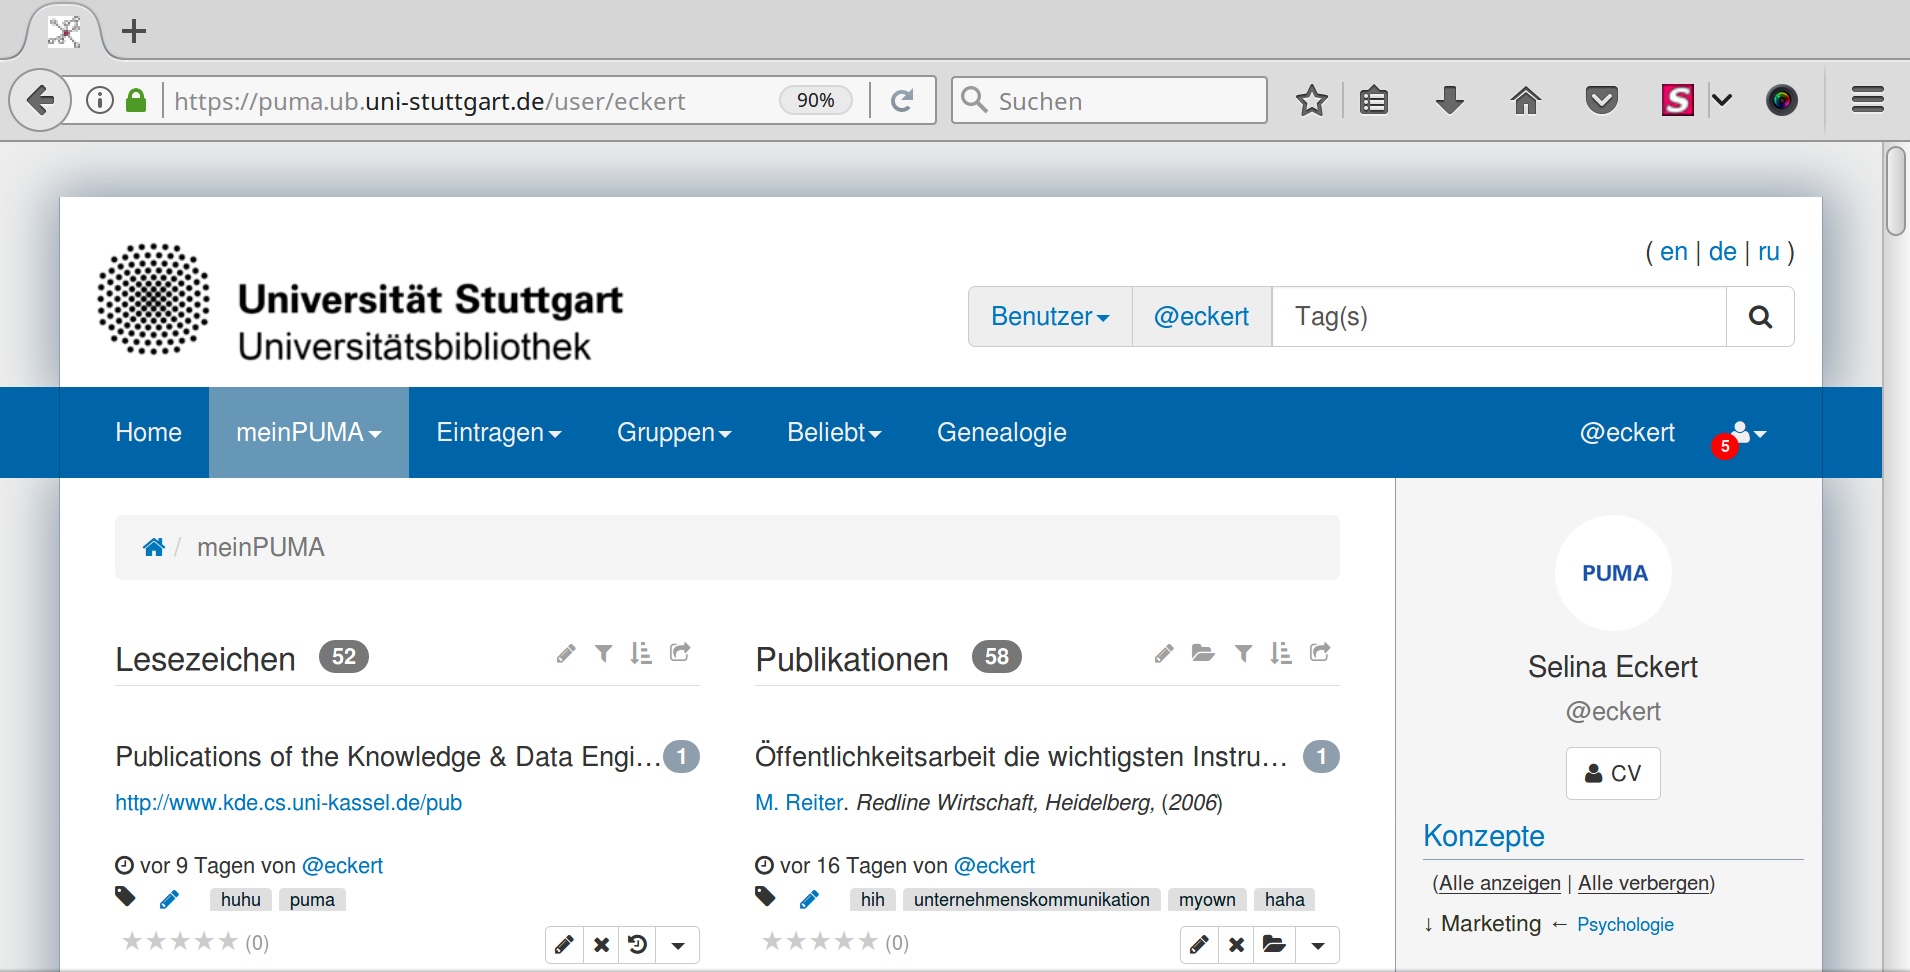
\includegraphics[width=11cm]{Bilder/Kapitel5/CV_Benutzerkonto}}
 %%\caption{Das Benutzerkonto}
 %%\label{fig:benutzerkonto}
%%\end{figure}  
%%Lebenslauf bearbeiten\index{Lebenslauf!bearbeiten}: 
%%\begin{enumerate}
    %%\item Klicken Sie auf Ihren Benutzernamen (@username).
    %%\item Klicken Sie rechts neben Ihrem Profilbild auf den CV-Button.
    %%\item Ihr Lebenslauf öffnet sich (Ansicht: So wie ihn andere Nutzer sehen).
    %%\item Um den Lebenslauf zu bearbeiten klicken Sie auf das schwarze Zahnrad neben \enquote{Curriculum Vitae}.
    %%\item Klicken Sie anschließend im Untermenü auf \enquote{Lebenslauf bearbeiten}. Sie können nun ein vordefiniertes Layout auswählen oder selbst ein Layout mit der MediaWiki-Syntax definieren.
%%\end{enumerate}
%%\textbf{Alternativer Weg:} 
%%\begin{enumerate}
    %%\item Klicken Sie auf das Personensymbol. Es öffnet sich ein Untermenü.
    %%\item Klicken Sie im Untermenü auf \enquote{Einstellungen}.
    %%\item Eine neue Seite öffnet sich. Klicken Sie auf den Reiter \enquote{Lebenslauf}. Sie können nun ein vordefiniertes Layout auswählen oder selber ein Layout mit der MediaWiki-Syntax definieren.
%%\end{enumerate}
%%\begin{wrapfigure}{l}{5cm}
%\begin{mdframed}[style=tipp]\texttt{Wenn Sie zwischen den vordefinierten Layouts wechseln, geht Ihr selbst definiertes Layout verloren.} \
%\end{mdframed}
%\todo{vielleicht zwei Styles Achtung und Tipp: Bin insgesamt mit dem Layout dieser Kästen nicht zufrieden}
%%\end{wrapfigure}
%\begin{figure}[h!]
 %\centering
 %\fbox{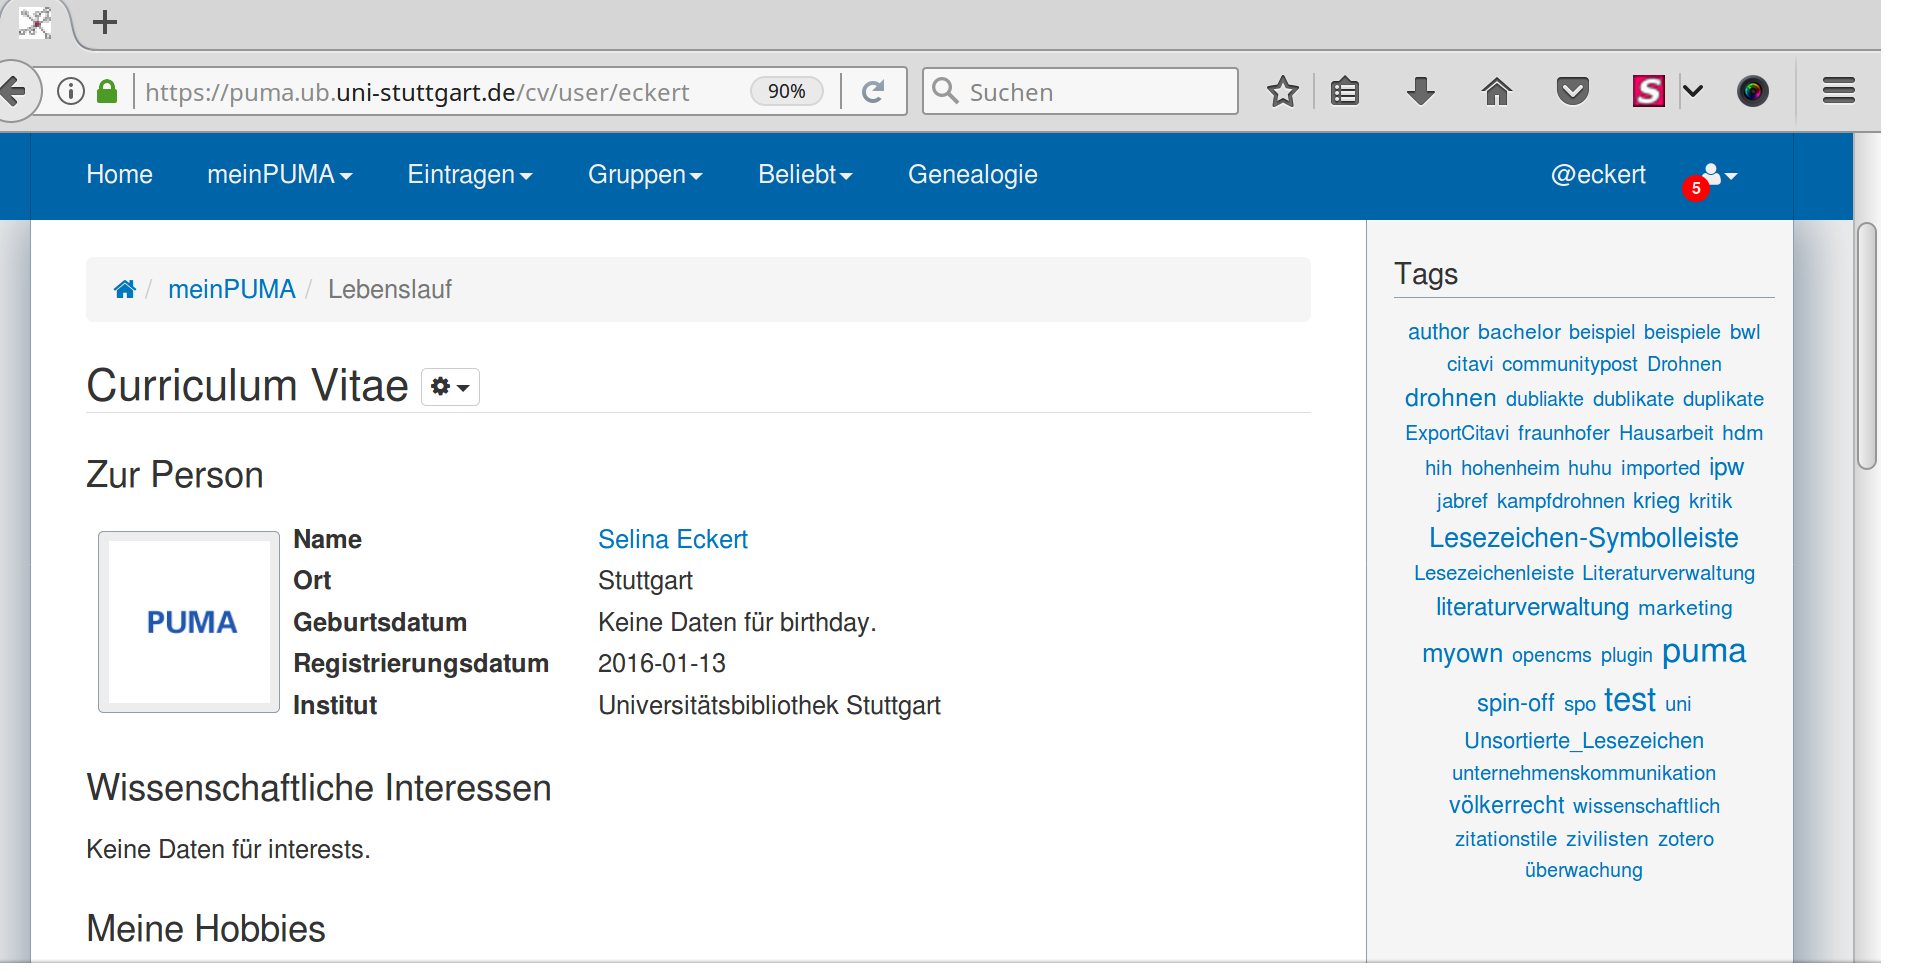
\includegraphics[width=11cm]{Bilder/Kapitel5/CV_Seite}}
 %\caption{Curriculum Vitae-Seite}
 %\label{fig:curriculumVitaeSeite}
%\end{figure}
%\todo[inline]{Bild ist veraltet, neuen Screenshot}
%\subsection{Eigenes Layout\index{Lebenslauf!Eigenes Layout}:}
%\label{subsec:eigenesLayout}
%Um sich selbst ein Layout zu definieren, wird die MediaWiki-Syntax verwendet. Dazu gibt es einige XHTML-Tags:
%\begin{figure}[h!]
 %\centering
 %\fbox{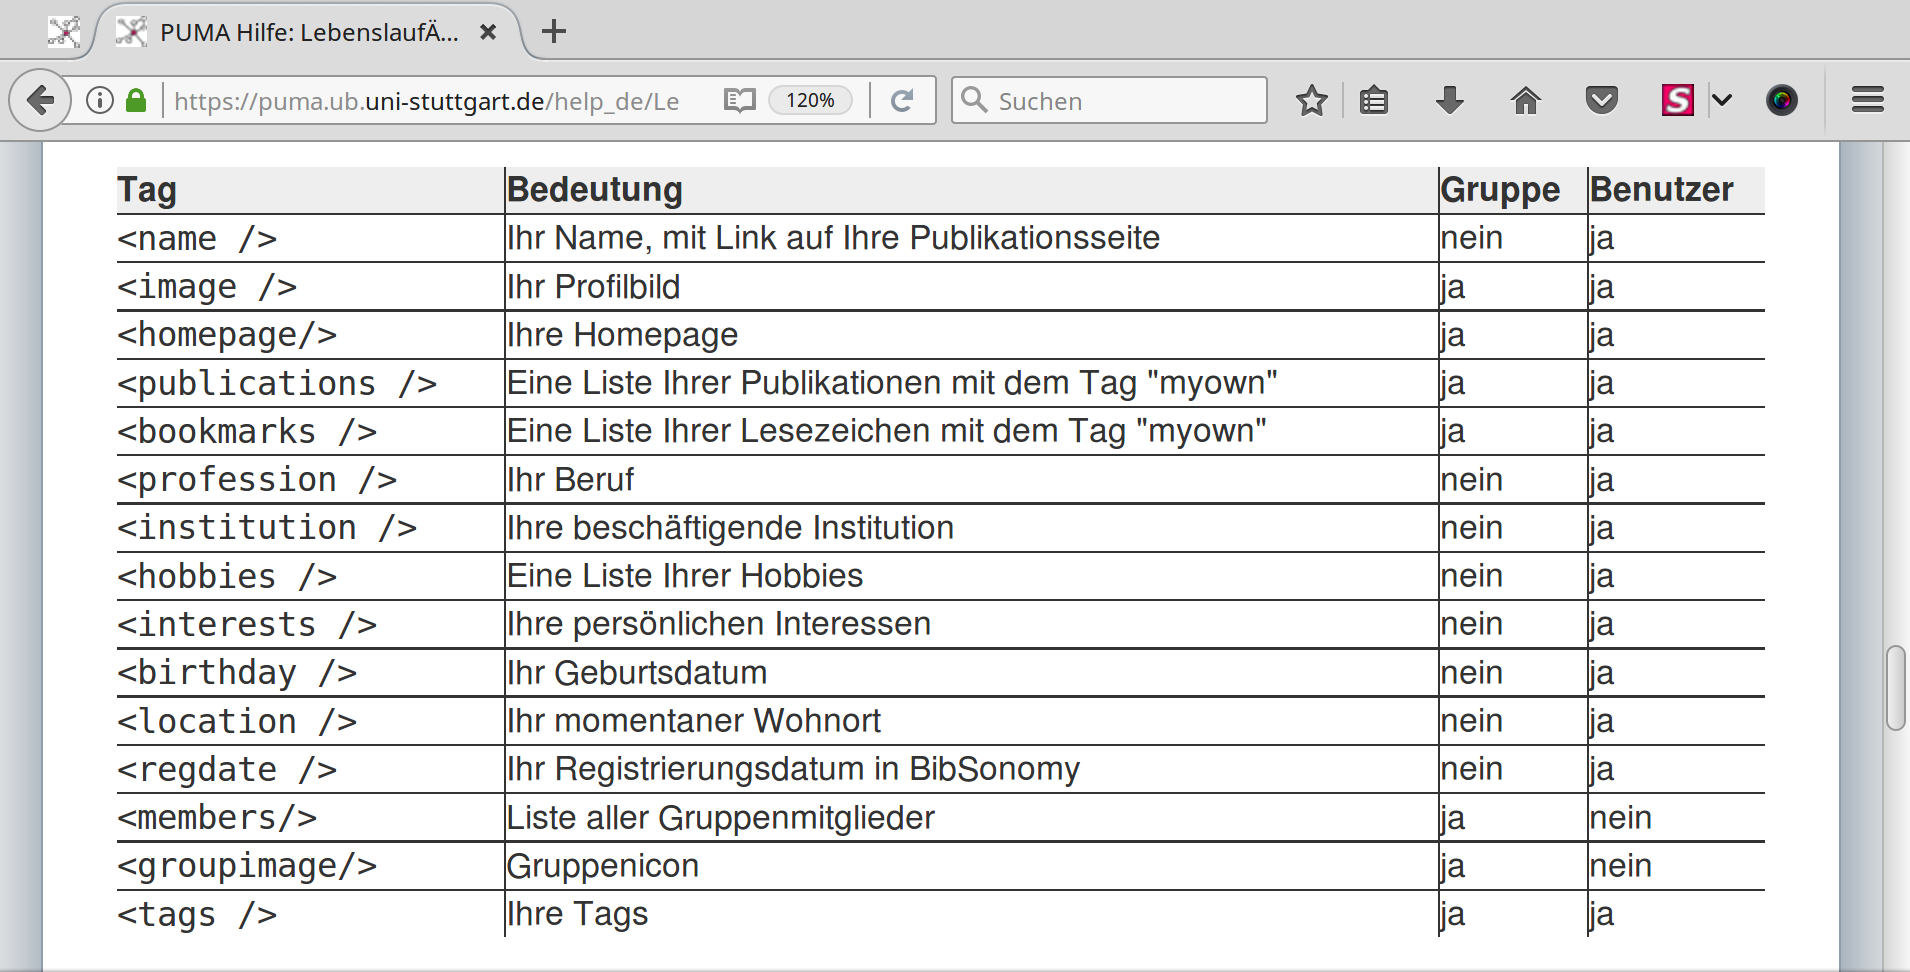
\includegraphics[width=11cm]{Bilder/Kapitel5/xhtml_tags}}
 %\caption{XHTML-Tags}
 %\label{fig:xhtmlTags}
%\end{figure} % Tabelle % ist XHTML bei wiki???
%\newline
%Für die Publikations- und Lesezeichenanzeige können außerdem zusätzliche Tags angegeben werden, um diese aus der eigenen Sammlung im Lebenslauf anzeigen zu lassen. Beispielsweise liefert \textit{<publications tags=\enquote{data mining} />} alle Publikationen, die sowohl mit data als auch mit mining getaggt wurden.  
\todo[inline]{Eigener Abschnitt zu Lebenslauf auskommentiert, ist das wirklich nötig? Eventuell noch oben ergänzen}
\section{Publikationen und Lesezeichen verwalten}
\label{sec:publikationen}
 Mit PUMA können sowohl Publikationen als auch Lesezeichen verwaltet werden. Es gibt verschiedene Wege Publikationen und Lesezeichen in PUMA einzutragen. Jede Publikation bzw. jedes Lesezeichen benötigt mindestens ein \tag. Mit Hilfe dieser \tags  werden die Einträge kategorisiert. Grundsätzlich sind alle Einträge öffentlich. Öffentliche Einträge sind auch für nicht angemeldete Nutzer sichtbar. Die Sichtbarkeit kann auf privat oder andere (Gruppen oder Freunde) eingeschränkt werden. 
\subsection{Publikationen}
\begin{figure}[htb]
 \centering
 \fbox{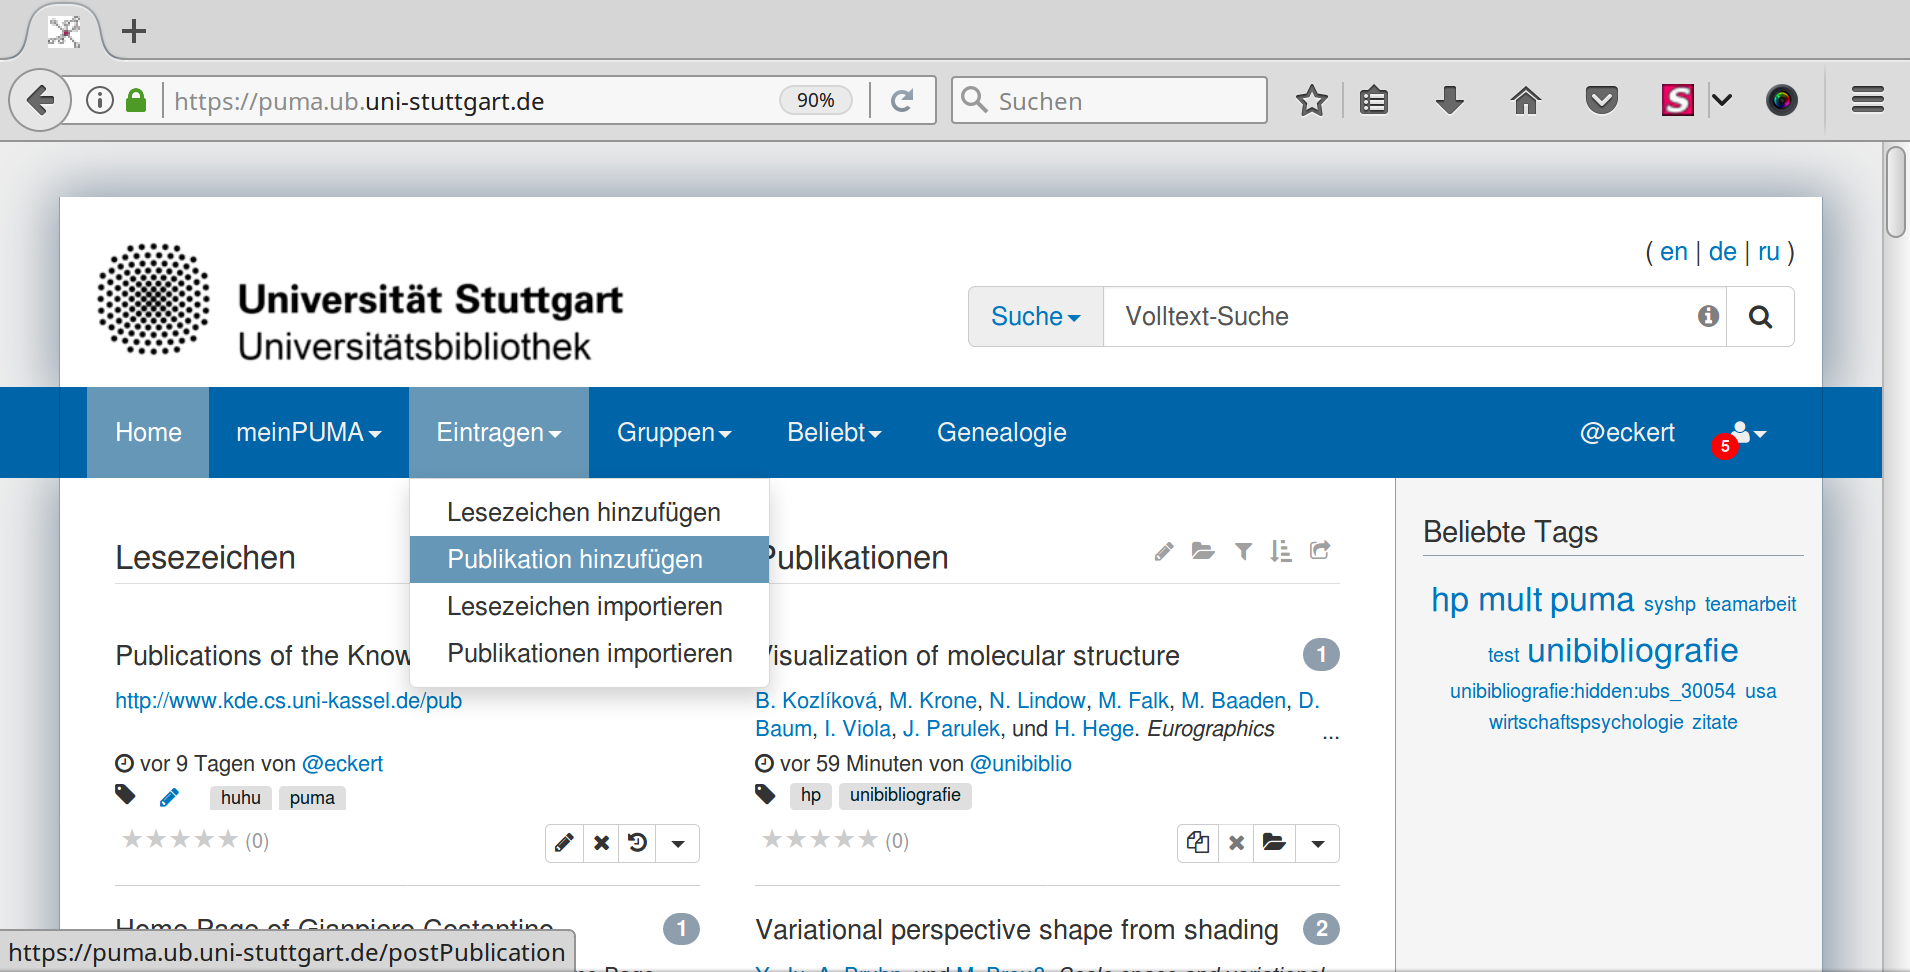
\includegraphics[width=11cm]{Bilder/Kapitel5/Publikation_eintragen}}
 \caption{Publikationen hinzufügen}
 \label{fig:publikationenHinzufügen}
\end{figure}  
Unter dem Menü \enquote{Eintragen} $\to$ \enquote{Publikation hinzufügen}\index{Publikationen!hinzufügen} kann direkt in das Textfeld der Titel oder die ISBN/~ISSN/~DOI der Publikationen eingeben werden. Des Weiteren gibt es zusätzliche Möglichkeiten Publikationen einzutragen:
%\begin{figure}[h!]
 %\centering
 %\fbox{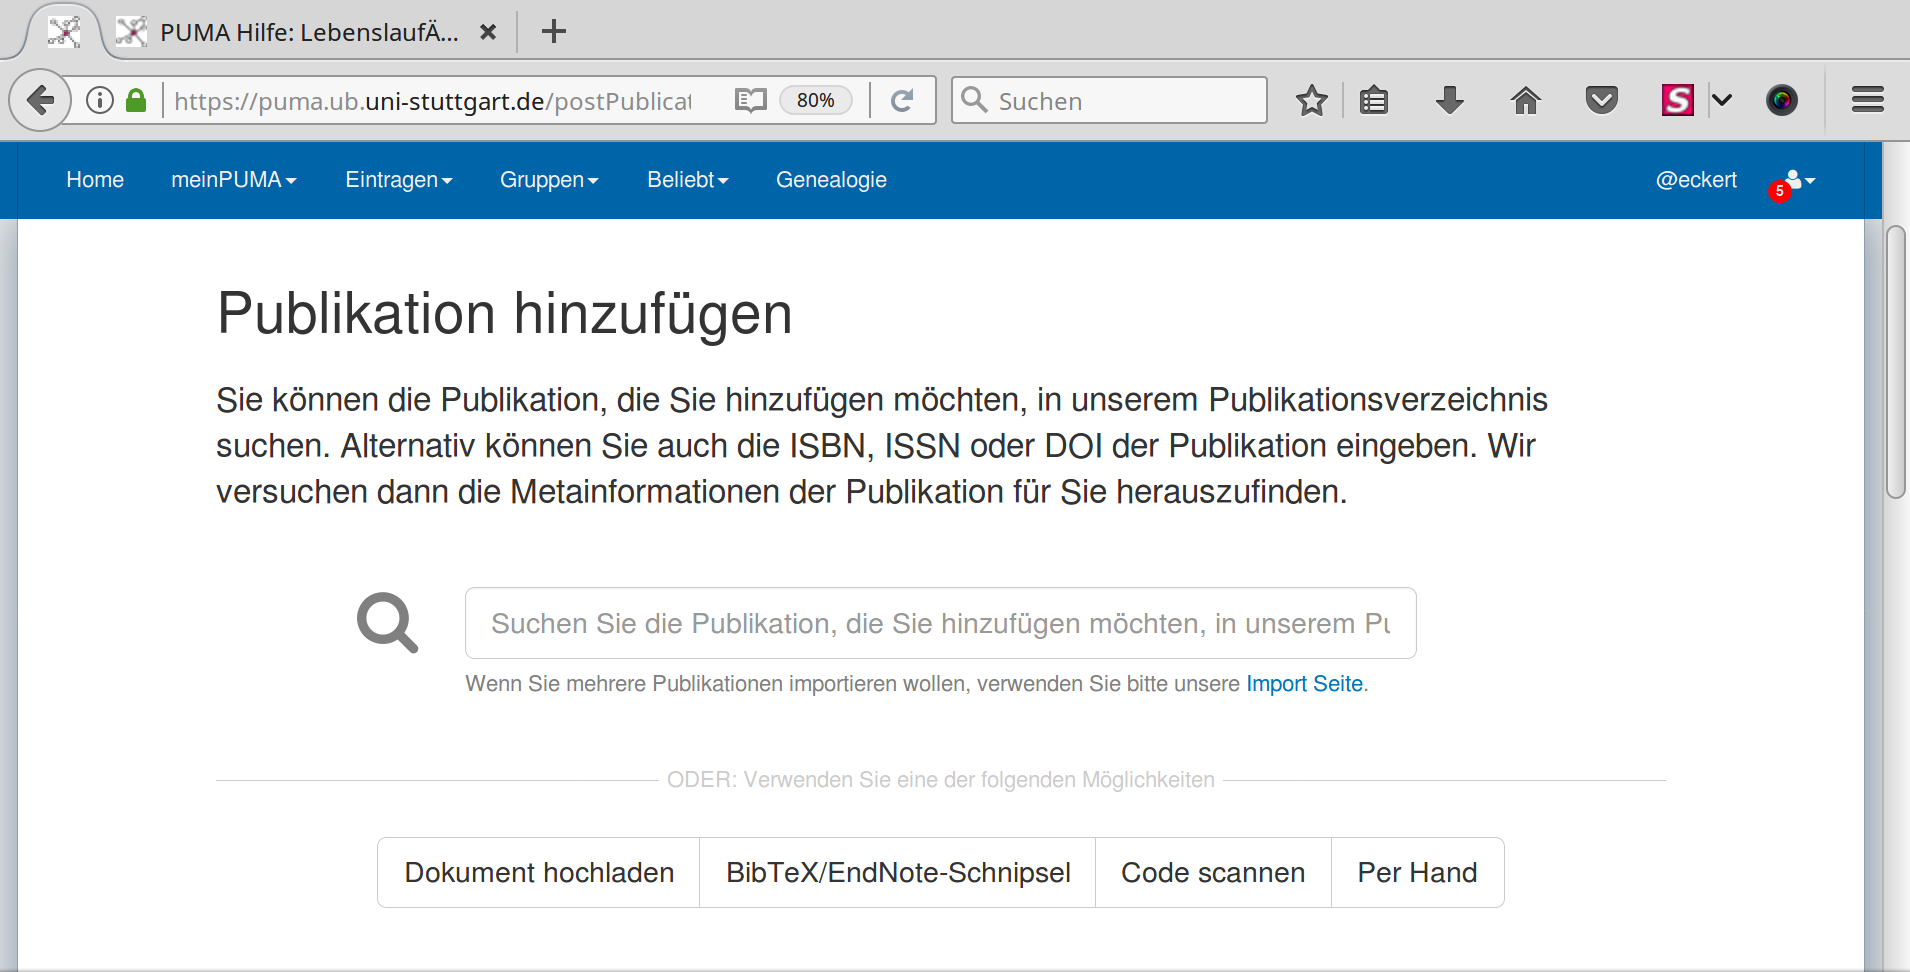
\includegraphics[width=11cm]{Bilder/Kapitel5/Eintragsmoeglichkeiten}}
 %\caption{Eintragsmöglichkeiten}
 %\label{fig:eintragungsmoeglichkeiten}
%\end{figure}  
    \begin{itemize}
    	\item Dokument hochladen:\newline
        Der Volltext einer Publikation kann hier hochgeladen werden. Das übliche Formular zum Eintragen (mit dem hoch geladenen Volltext) der Publikationen öffnet sich. Einige Felder sind bereits ausgefüllt und können ergänzt werden.
				\begin{tip}
Achtung Betaversion! Diese Funktion befindet sich gerade in der Entwicklung.
\end{tip}
			\item BibTex\index{BibTex}/EndNote\index{EndNote}-Schnipsel:\newline
			Kopierte Zitationen können hier eingefügt werden. Diese Informationen werden dann übernommen und können ergänzt werden.
        \item Code scannen\index{Code Scannen}: \newline
Über eine Webcam kann der Barcode gescannt werden. Ggf. muss der Zugriff von PUMA auf die Webcam erlaubt werden. Sobald der Barcode erkannt wurde, werden die Daten angezeigt und können ergänzt werden
        \item Per Hand:
				Hier kann der Eintragstyp, Titel, Autor(en), Herausgeber und Jahr der Publikation eingetragen werden. Mit \enquote{Weiter} erscheinen alle Felder der Eingabemaske. \todo{Verweis auf Eintragstypen}
    \end{itemize}
\begin{tip} Über die Url \url{https://puma.ub.uni-stuttgart.de/editPublication} kann direkt auf die erweiterte Eingabemaske zugegriffen werden
\end{tip}		
%\begin{figure}[h!]
 %\centering
 %\fbox{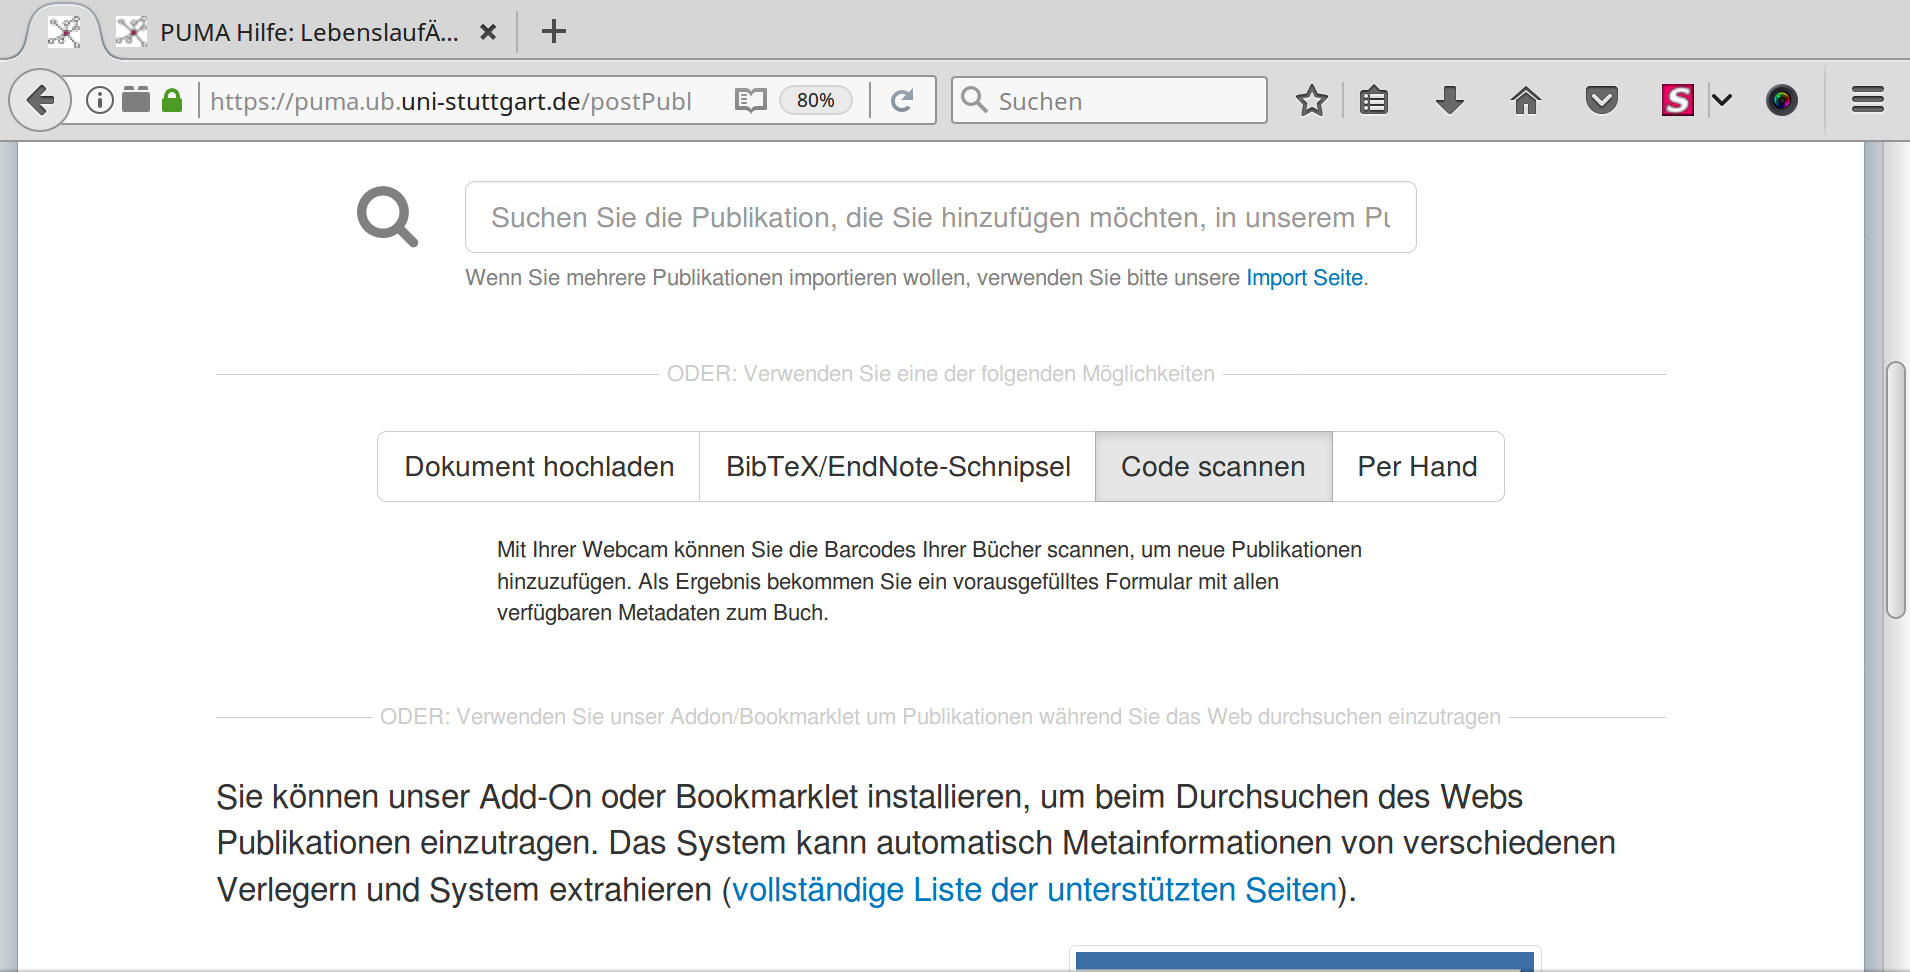
\includegraphics[width=11cm]{Bilder/Kapitel5/Code_scannen}}
 %\caption{Code scannen}
 %\label{fig:codeScannen}
%\end{figure}
Über \enquote{Eintragen} $\to$ \enquote{Publikation importieren} kann eine Text-Datei hochgeladen werden. Folgende Aktionen können bei den Einträgen der Datei in PUMA ausgewählt werden:
\begin{tip}
Bei EndNote wird beim Speichern eine Datei mit der Endung .enl erzeugt, diese enthält die komplette Datenbank. Für den Import in PUMA sollte ein Textdatei importiert werden. Dazu muss die Datei in EndNote nicht speichern, sondern exportieren. PUMA kann mit verschiedenen Formaten umgehen. Um BibTex zu exportieren muss der Output-Stil angepasst werden. Wenn BibTex nicht angezeigt wird, unter \enquote{Edit} $\to$ \enquote{Output-Styles} $\to$ \enquote{Open Style Manager} BibTex aus der Liste auswählen. Über \enquote{File} $\to$\enquote{Export} den \enquote{BibTex Export} auswählen. Beim Speichern \enquote{Text only} auswählen und die Datei mit der Endung .bib speichern.
\end{tip}
Nach dem Hochladen stehen verschiedene Möglichkeiten zur Verfügung die Einträge weiter zu bearbeiten:
\begin{itemize}
\item Tags zu allen ausgewählten Einträgen hinzufügen: An jeden Eintrag wird der gleiche \tag hinzugefügt
\item Die Tags aller ausgewählten Einträge separat bearbeiten: \tags können auch an einzelne Einträge hinzugefügt werden
\item BibTeX-Schlüssel normalisieren: BibTex-Schlüssel werden nach dem Schema NameJahrTitel normalisiert, wobei Name der Nachname des primären Autors , Jahr das Jahr der Veröffentlichung und Titel das erste Wort des Titels der Publikation ist, das mehr als fünf Buchstaben enthält. Beispiel: knuth1998programming.
\item Sichtbarkeit einstellen: öffentlich, privat oder für Freunde \todo{referenz und erklärung ergänzen}
\end{itemize}
\begin{tip} Einträge, die bereits in der eigenen Sammlung vorhanden sind, werden als Fehler angezeigt. Wenn alte Einträge überschrieben werden sollen, kann dies vor dem hochladen der Datei ausgewählt werden.
\end{tip}
\subsection{Lesezeichen} % 2Screenshots: Anfang+Möglichkeiten
\label{subsec:lesezeichen}
Die URL eines Lesezeichen \index{Lesezeichen!hinzufügen} kann über den Menüpunkt \enquote{Eintragen} $\to$ \enquote{Lesezeichen hinzufügen} hinzugefügt werden. 
\begin{figure}[h!]
 \centering
 \fbox{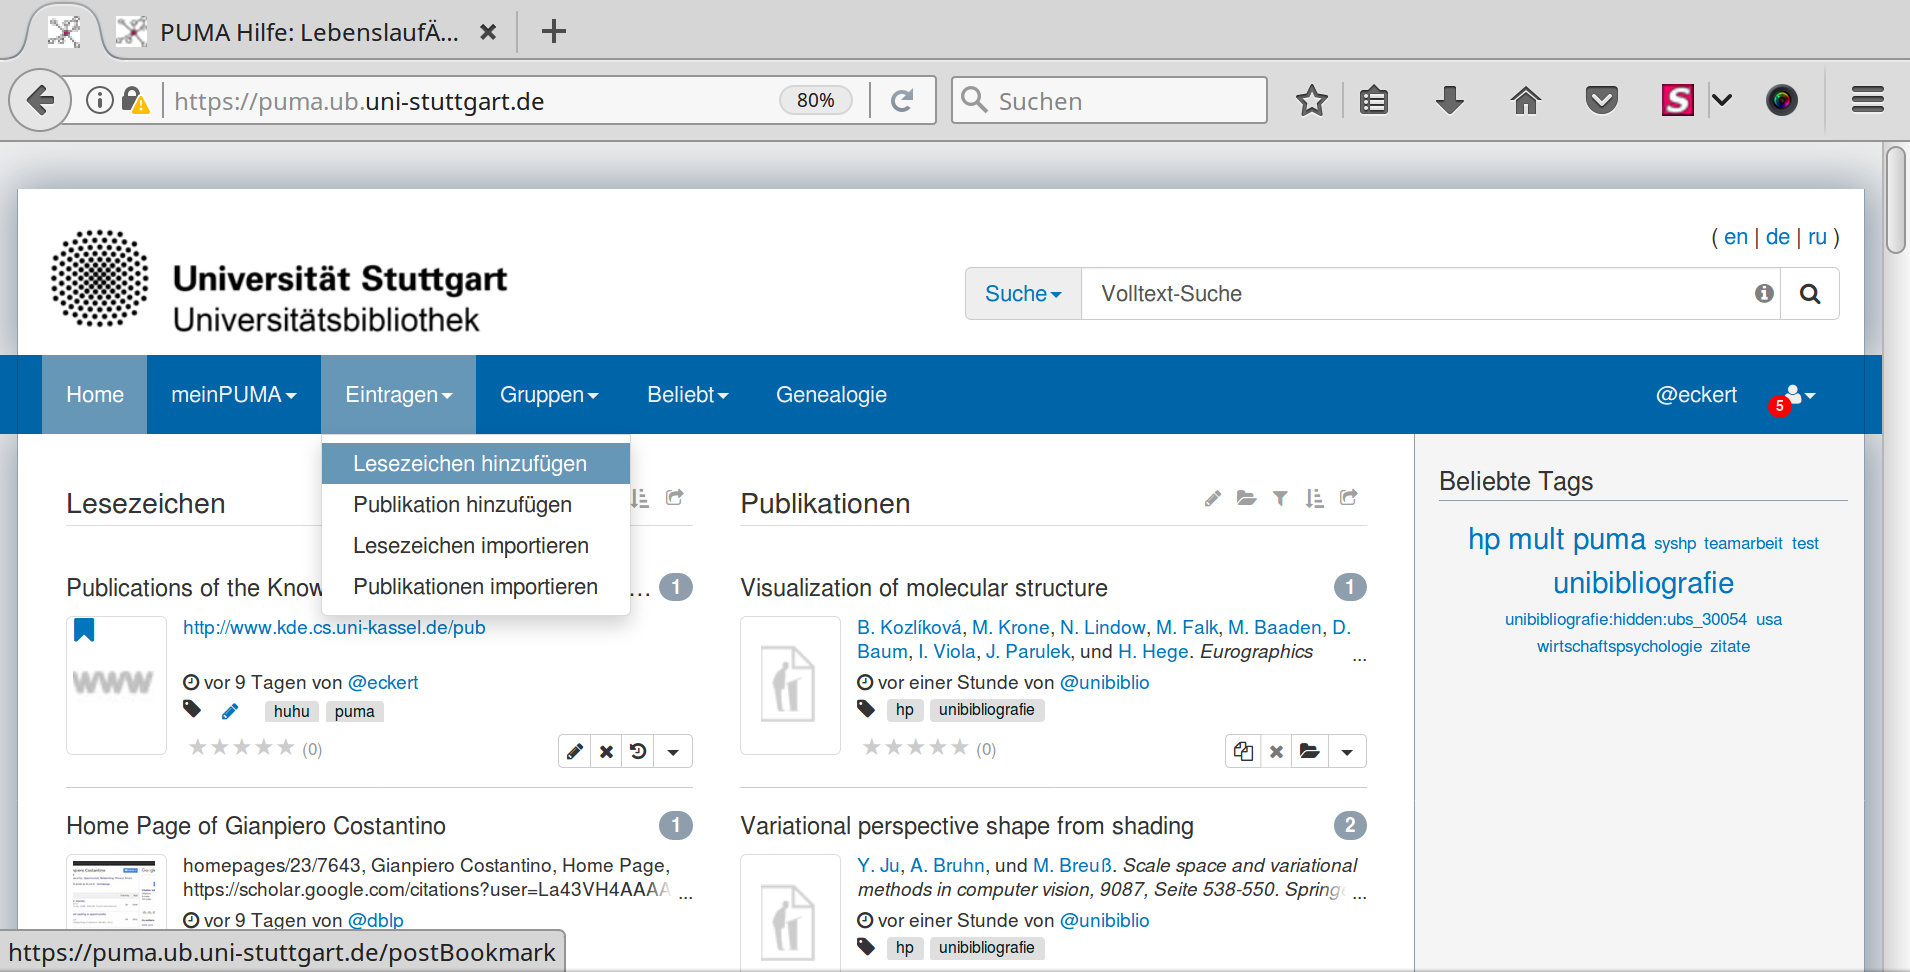
\includegraphics[width=11cm]{Bilder/Kapitel5/Lesezeichen_hinzufuegen}}
 \caption{Lesezeichen hinzufügen}
 \label{fig:lesezeichenHinzufuegen}
\end{figure}  
\underline{Wichtig bei der Recherche und Archivierung von Lesezeichen:}
\begin{itemize}
    \item Puma speichert nicht das eigentliche Dokument, sondern nur die Adresse des Internet-Dokuments. Es kann somit passieren, dass ein Dokument zu einem späteren Zeitpunkt nicht mehr abrufbar ist, da z.B. sich die Adresse geändert hat oder es gelöscht wurde.  
    \item In der Literaturangabe zu einem Internet-Dokument sollte immer das Datum des letzten Abrufs mit angegeben werden. Folgende Möglichkeiten bieten sich an dies in der Literaturliste anzupassen: Die Lesezeicheneinträge werden beim BibTeX-Export als \enquote{electronic} exportiert. Entweder diese Liste für die Literaturangaben manuell im Dokument anpassen, im dem man das \enquote{added-on} Feld in das Bibtex-Feld \enquote{urldate} umbenennt\autocite[Vgl. das Benutzerhandbuch zum BibLaTeX Paket][S.10 (der Eingabetyp \enquote{online} wird synonym zu \enquote{electronic} verwendet. Damit der Zitationsstil das Abrufdatum hinzufügt muss das Feld urldate ausgefüllt sein.)]{lehmann2016biblatex}
    \item PUMA unterstützt die RFC 7089\footnote{\url{http://tools.ietf.org/html/rfc7089}} Spezifikation\index{RFC 7089 Spezifikation}. Damit wird es möglich, Lesezeichen so zu betrachten, wie sie in PUMA gespeichert wurden, selbst wenn sich die Seite in der Zwischenzeit geändert hat. Um diese Funktion zu nutzen, müssen Sie das Memento-Plugin in ihrem Browser installieren. Das Plugin existiert für Mozilla Firefox\footnote{\url{https://addons.mozilla.org/de/firefox/addon/mementofox/}} und Google Chrome\footnote{\url{https://chrome.google.com/webstore/detail/memento-time-travel/jgbfpjledahoajcppakbgilmojkaghgm?hl=en&gl=US}}. \todo{auf Marios anwort warten}
\end{itemize}
\section{Versionierung der Publikationen und Lesezeichen}
\label{sec:versionierung}
Publikationen und Lesezeichen können jederzeit eingetragen und bearbeitet werden. Um sich einen Überblick über die vorgenommen Änderungen zu verschaffen, bietet PUMA eine Versionsgeschichte\index{Versionierung} zu jeder Publikation und jedem Lesezeichen an. Klicken Sie in Ihrer eigenen Sammlung auf den kleinen schwarzen Pfeil neben einer beliebigen Publikation. Es öffnet sich ein Dropdown-Menü, in dem Sie \enquote{Verlauf dieser Publikation} auswählen. Ihnen wird sofort die Versionsgeschichte der jeweiligen Publikation/~Lesezeichen angezeigt und Sie können jede Ihrer Änderungen nachverfolgen. 
\begin{figure}[h!]
 \centering
 \fbox{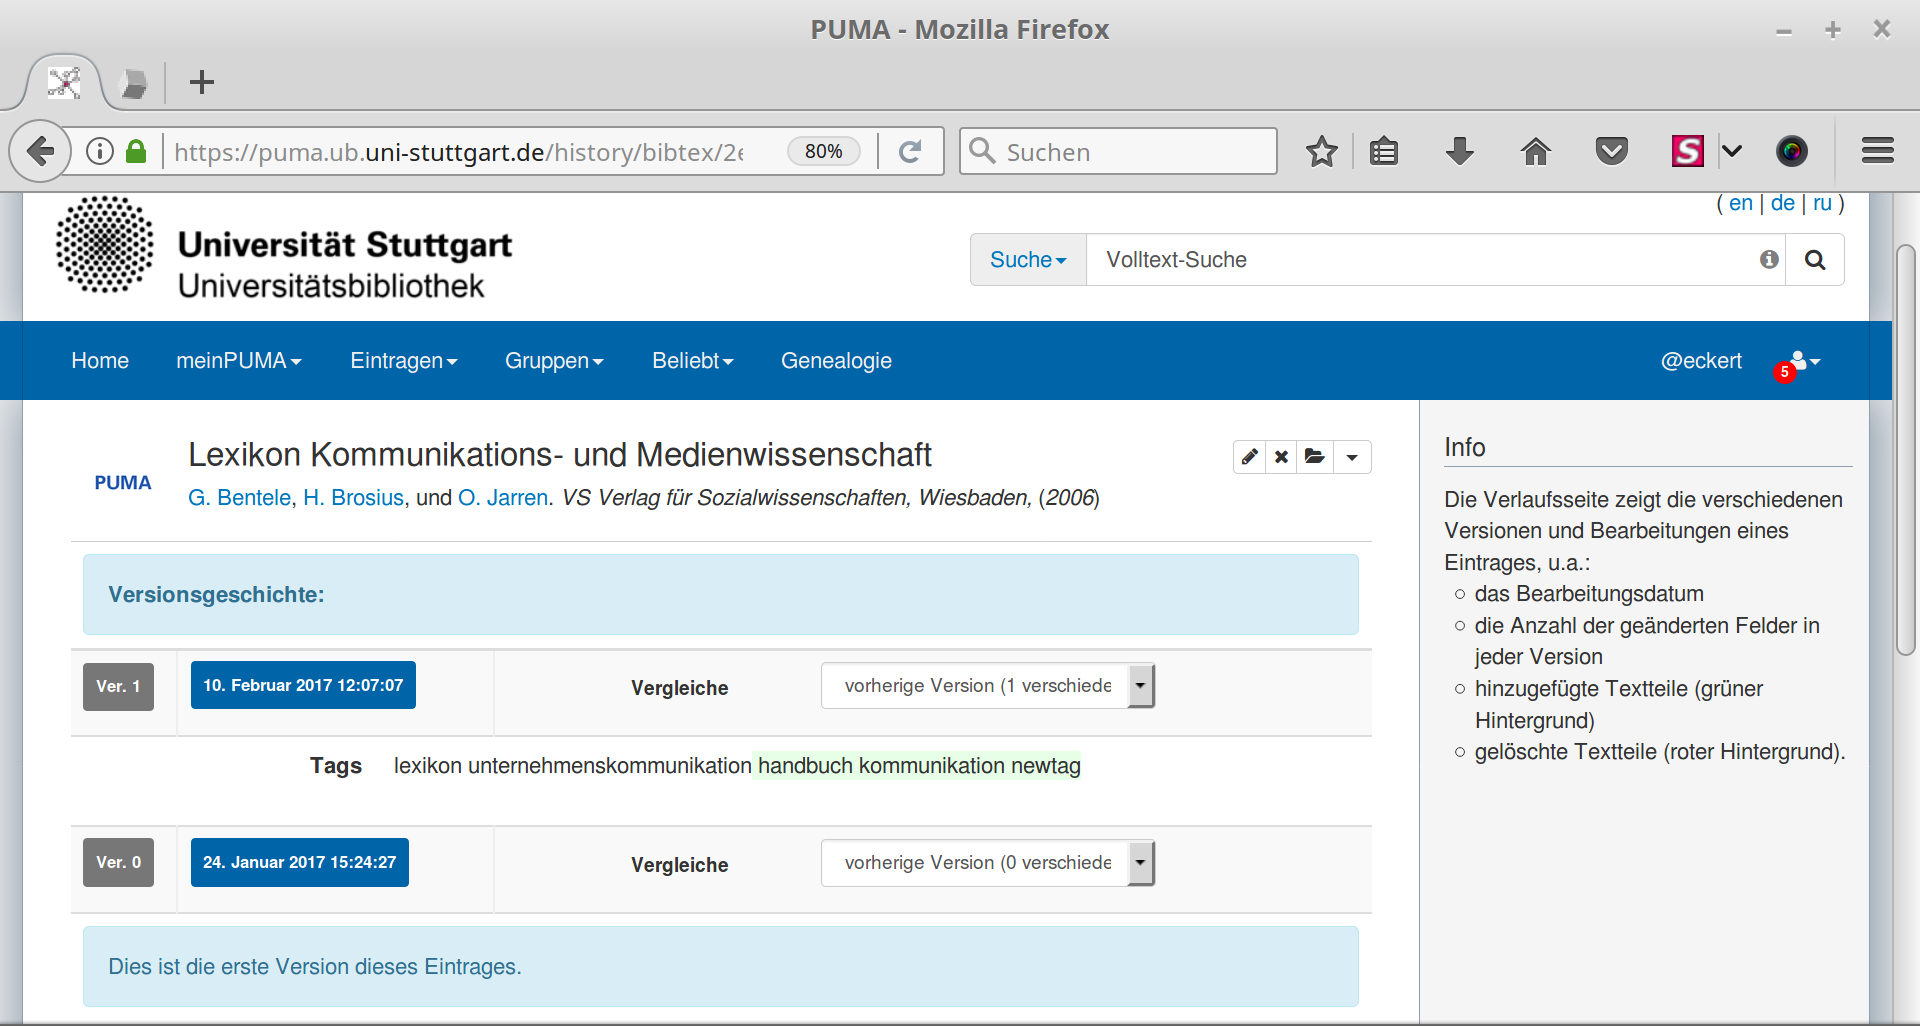
\includegraphics[width=9cm]{Bilder/Kapitel5/Versionsgeschichte}}
 \caption{Die Versionsgeschichte}
 \label{fig:versionsgeschichte}
\end{figure} 
\section{Lesezeichen importieren}
\label{sec:lesezeichenImportieren}
\subsection{Browser}
\label{subsec:browser}
PUMA ermöglicht es Ihnen HTML-Dateien in PUMA zu importieren. Hierfür exportieren Sie ihre Lesezeichen aus ihrem Browser als HTML-Datei und importieren diese anschließend. Je nach Browser unterscheidet sich das Exportieren der Lesezeichen.
\newline
\newline
\textbf{Chrome}%Screenshots hab ich schon
\newline Um ihre Lesezeichen in Chrome\index{Chrome} als HTML-Datei zu exportieren, klicken Sie im Menü oben rechts auf \enquote{Lesezeichen} und anschließend auf \enquote{Lesezeichen-Manager}. Es öffnet sich ein neues Fenster, in dem Sie auf \enquote{Organisieren} klicken und im Dropdown-Menü \enquote{Lesezeichen in HTML-Datei exportieren...} wählen. Speichern Sie die Datei ab und fahren mit Schritt 1 von HTML-Datei in PUMA importieren fort, um Ihre Lesezeichen endgültig nach PUMA zu importieren.  
\begin{figure}[h!]
 \centering
 \fbox{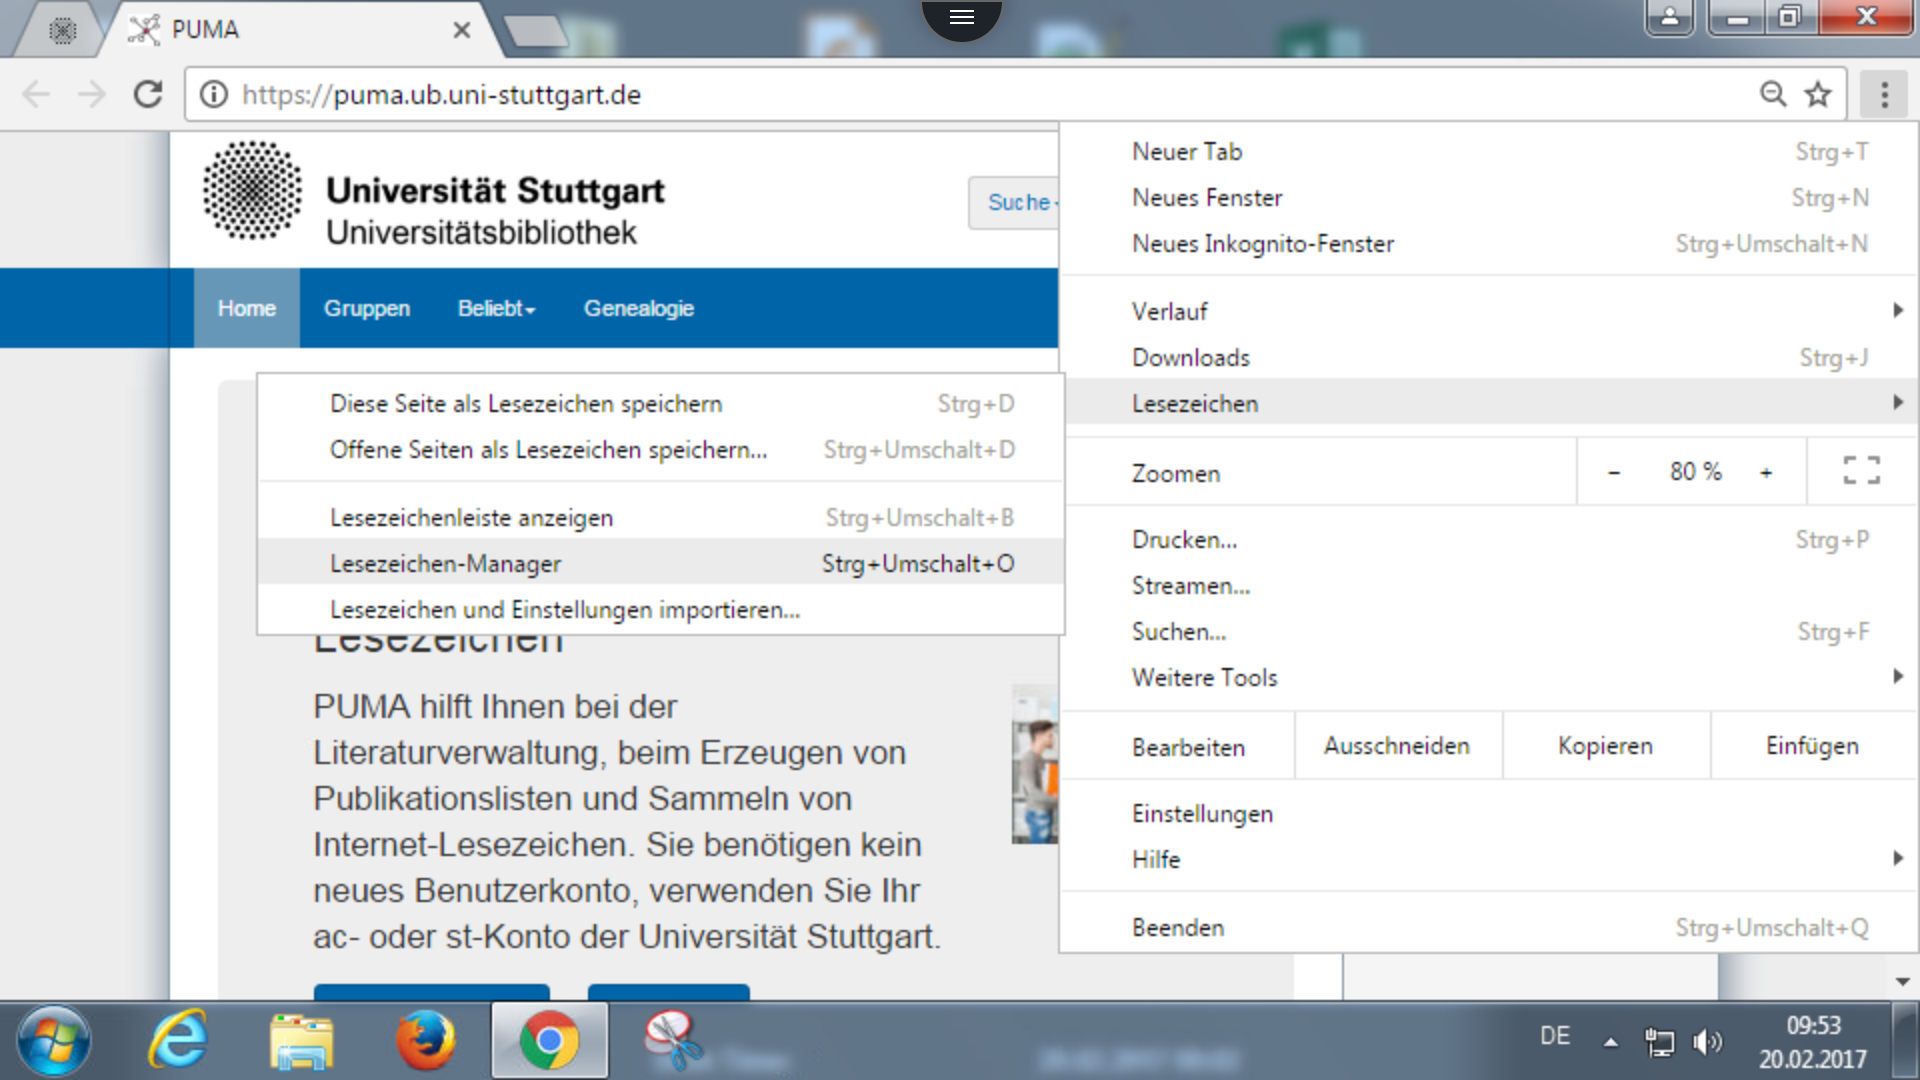
\includegraphics[width=11cm]{Bilder/Kapitel5/Lesezeichen-Manager_Chrome}}
 \caption{Der Lesezeichen-Manager}
 \label{fig:lesezeichenManager}
\end{figure}
\begin{figure}[ht]
 \centering
 \fbox{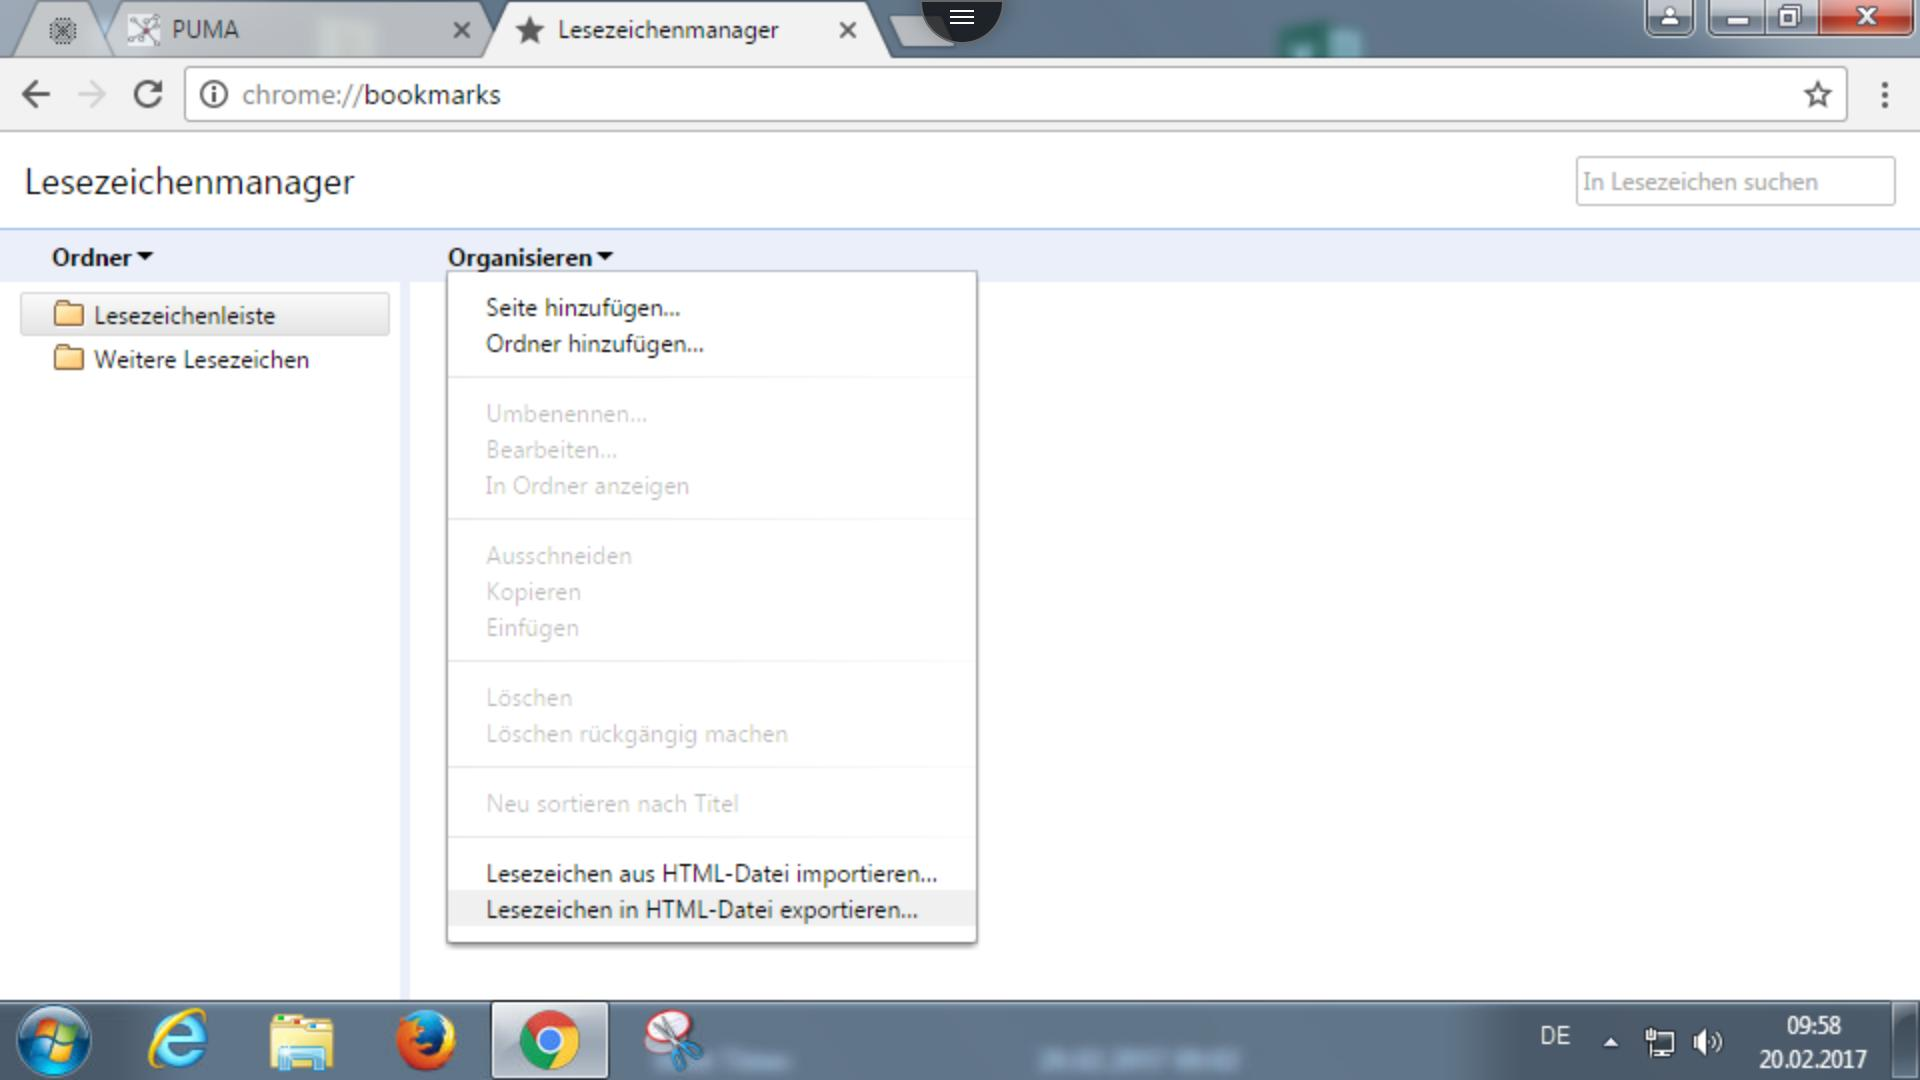
\includegraphics[width=9cm]{Bilder/Kapitel5/Lesezeichen_HTML_Chrome}}
 \caption{Lesezeichen in HTML-Datei exportieren}
 \label{fig:lesezeichenHtmlExportieren}
\end{figure}

\textbf{Firefox}
\newline Um Ihre Lesezeichen in Firefox\index{Firefox} als HTML-Datei zu exportieren, klicken Sie auf das Lesezeichensymbol rechts neben der Suchleiste. Wählen Sie im Dropdown-Menü \enquote{Lesezeichen verwalten} aus.

\begin{figure}[h!]
 \centering
 \fbox{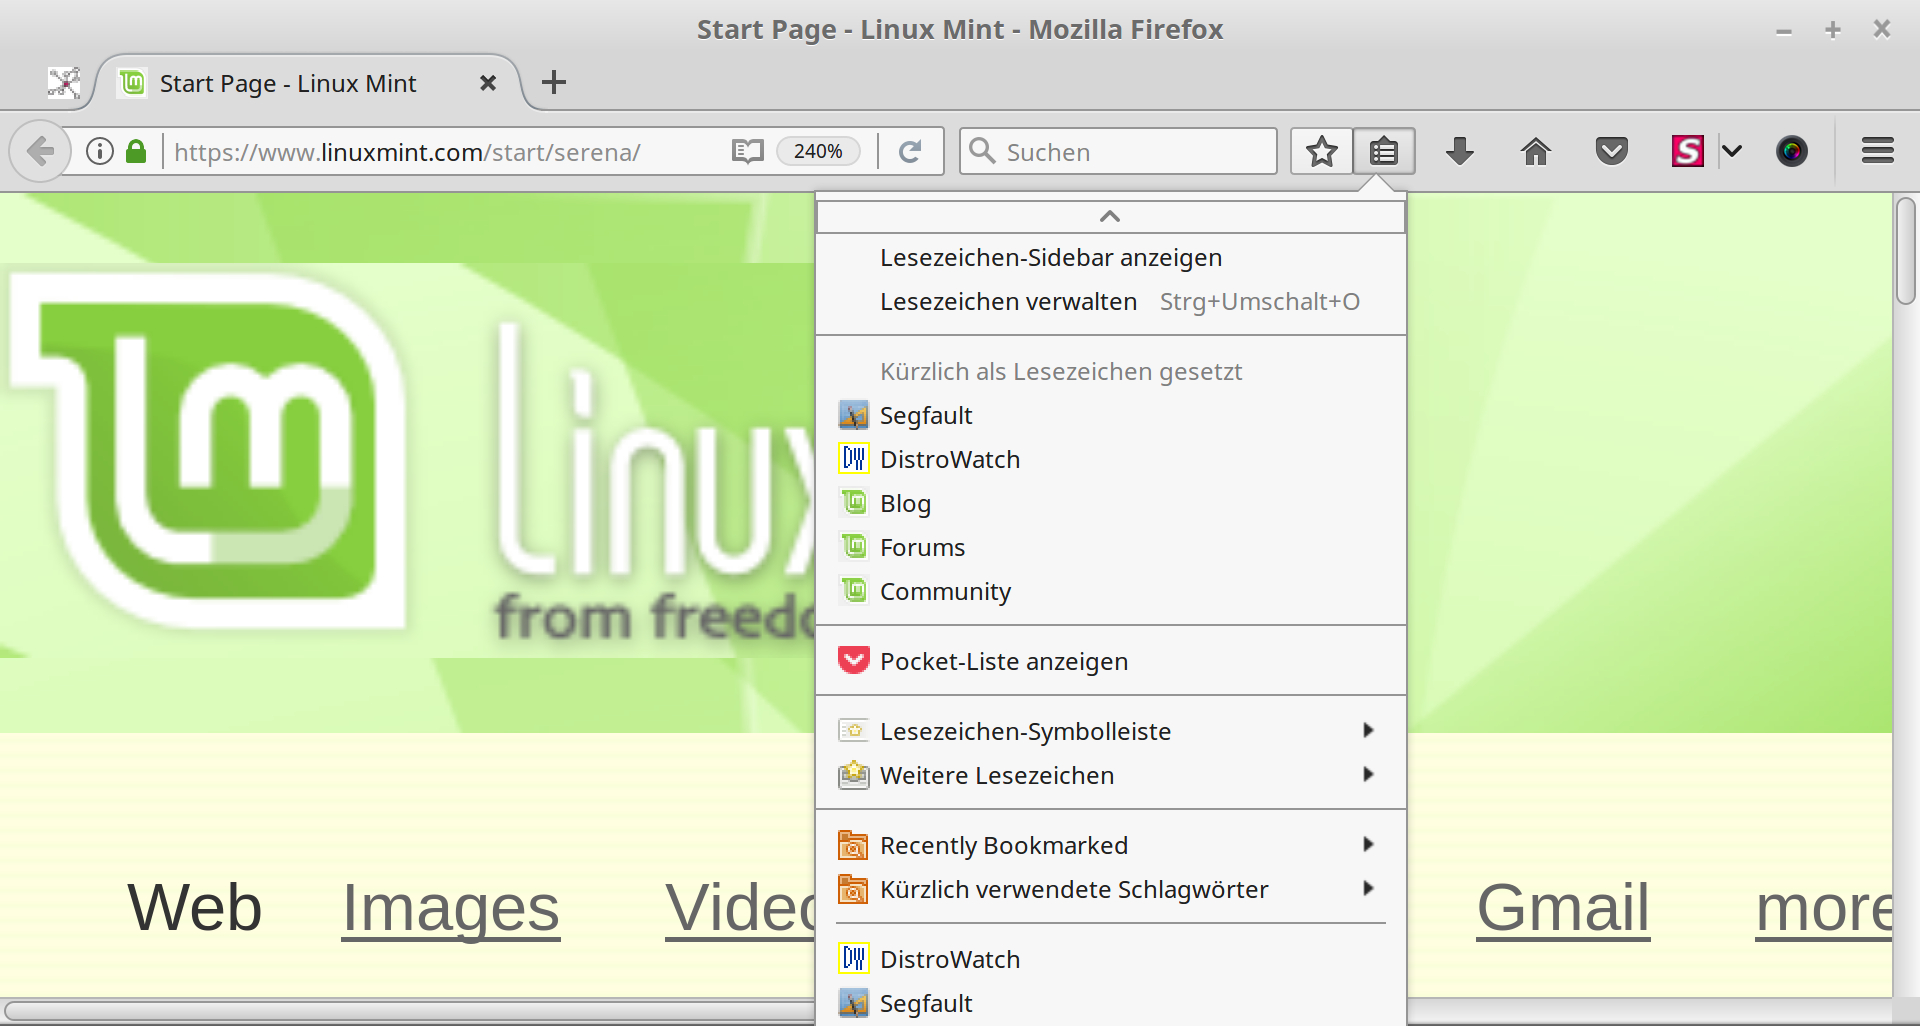
\includegraphics[width=11cm]{Bilder/Kapitel5/Firefox_Lesezeichen_verwalten}}
 \caption{Lesezeichen verwalten}
 \label{fig:lesezeichenVerwalten}
\end{figure}
Anschließend klicken Sie auf \enquote{Importieren und Sichern} und wählen \enquote{Lesezeichen nach HTML exportieren} aus. Speichern Sie die Datei ab und fahren mit Schritt 1 von HTML-Datei in PUMA importieren fort, um Ihre Lesezeichen endgültig nach PUMA zu importieren.  

\begin{figure}[h!]
 \centering
 \fbox{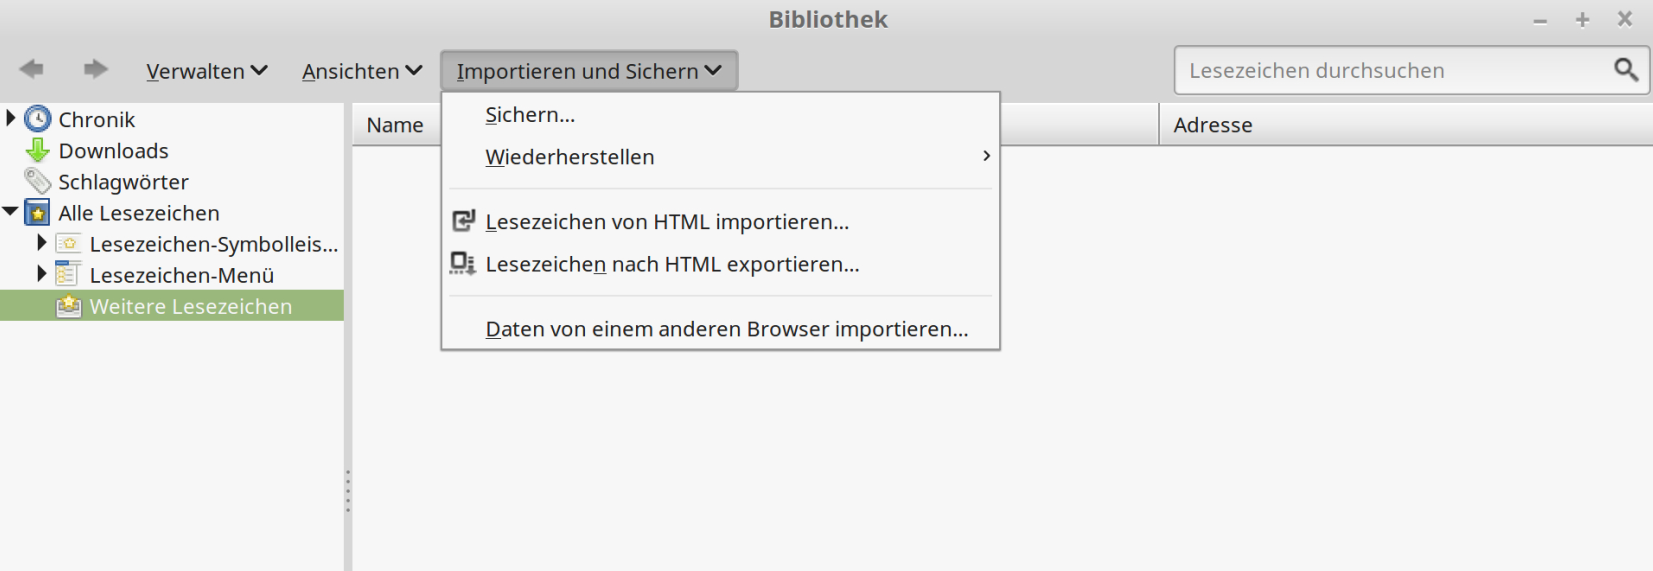
\includegraphics[width=11cm]{Bilder/Kapitel5/Firefox_Importieren_Speichern}}
 \caption{Importieren und Sichern}
 \label{fig:importierenSichern}
\end{figure}
\subsection{HTML-Datei\index{HTML-Datei} in PUMA importieren}
\label{subsec:htmlDateiImportieren}
\begin{enumerate}
    \item Klicken Sie auf \enquote{Eintragen} und wählen im Dropdown-Menü \enquote{Lesezeichen importieren} aus.
    \item Es öffnet sich eine neue Seite. In dem Bereich \enquote{Importieren Sie Ihre Lesezeichen aus Ihrem Browser} können Sie nun die entsprechende Datei hochladen. 
    \item Legen Sie die Sichtbarkeit der Lesezeichen fest und bestätigen Sie Ihren Import anschließend mit \enquote{Importieren}.
\end{enumerate}
\begin{figure}[h!]
 \centering
 \fbox{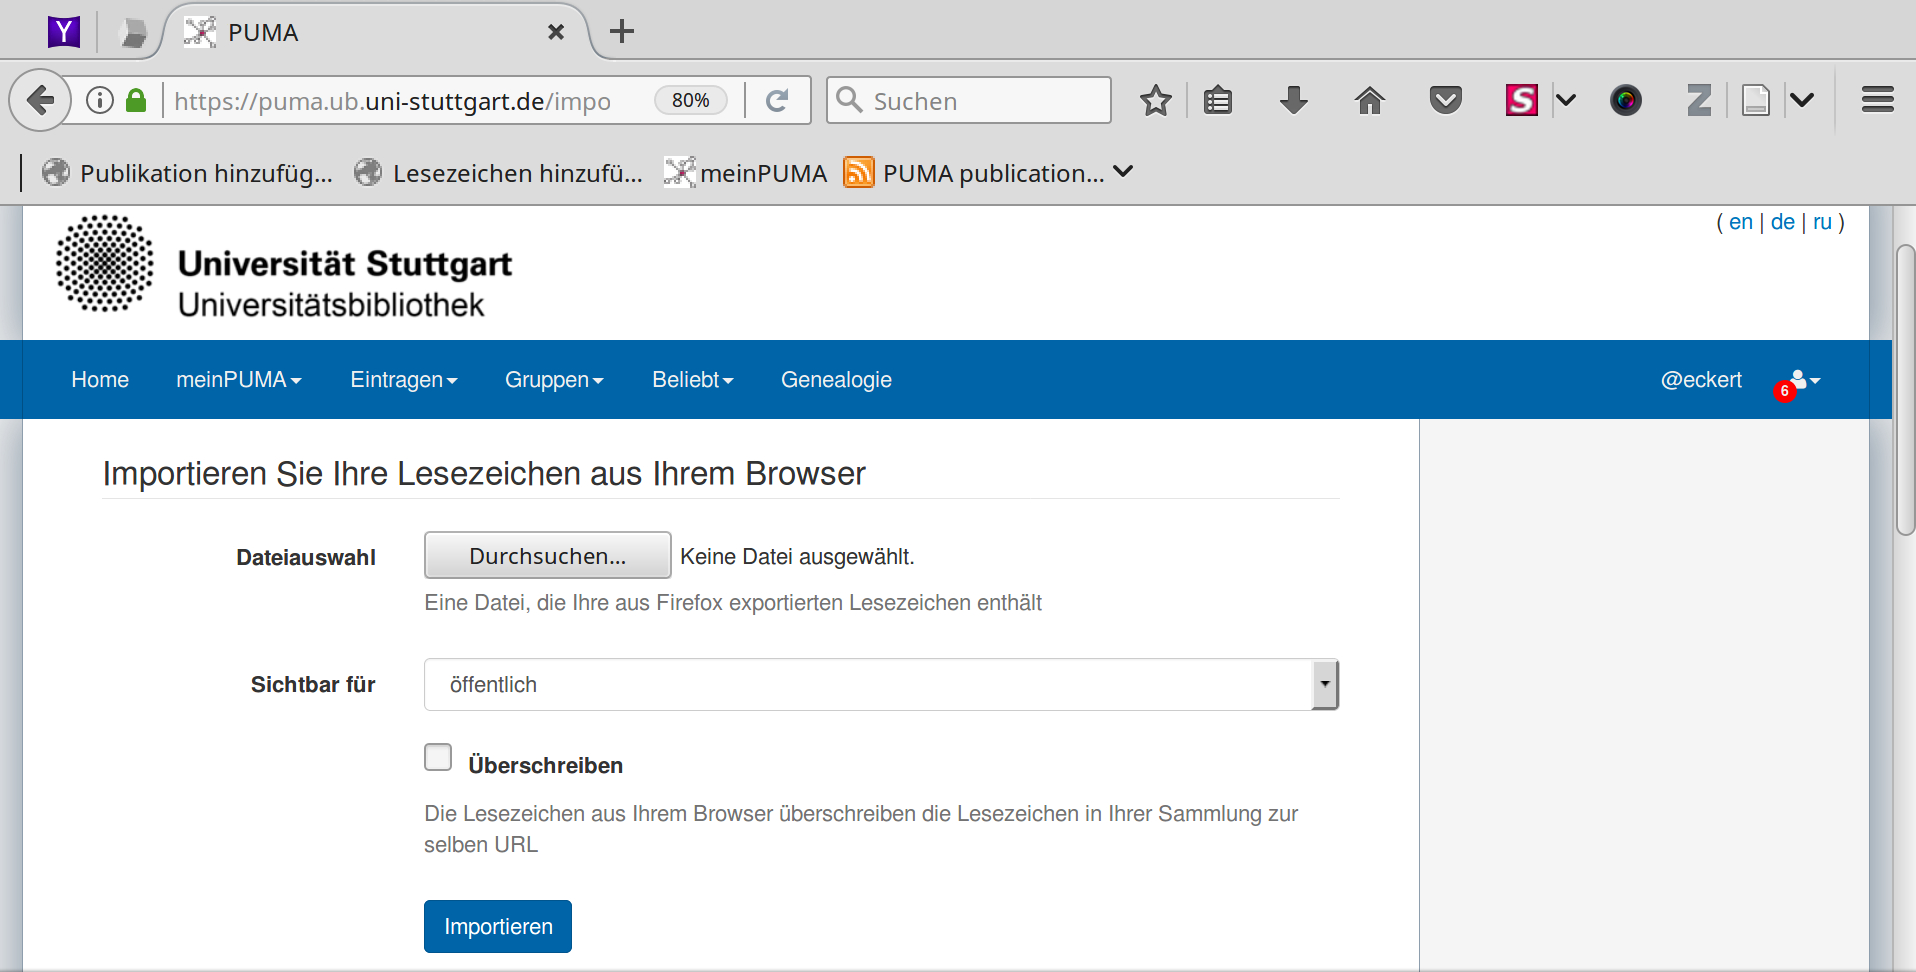
\includegraphics[width=11cm]{Bilder/Kapitel5/HTML-Datei_hochladen}}
 \caption{HTML-Datei hochladen}
 \label{fig:htmlDateiHochladen}
\end{figure}
\subsection{Delicious}
\label{subsec:delicious}
Sie möchten Ihre Lesezeichen von Delicious\index{Delicious} nach PUMA importieren. Klicken Sie auf \enquote{Eintragen} und wählen im Dropdown-Menü \enquote{Lesezeichen importieren} aus. Geben Sie unter dem Bereich \enquote{Importieren Sie Ihre Delicious Daten} Ihre Delicious-Nutzerdaten ein. \newline
Legen Sie im darauffolgenden Schritt fest, ob Ihre Delicious Lesezeichen bereits vorhandene Lesezeichen in Ihrer Sammlung mit der selben URL überschreiben sollen.\newline
Sie können im letzten Schritt festlegen, ob Sie Ihre Lesezeichen oder Tag-Bundles importieren möchten. Wenn Sie die Option \enquote{Lesezeichen} wählen, werden zusammen mit Ihren Lesezeichen die dazugehörigen Tags und Sichtbarkeitsdefinitionen mit übernommen.
\newline Klicken Sie abschließend auf \enquote{Importieren} um den Import endgültig durchzuführen.
\begin{figure}[h!]
 \centering
 \fbox{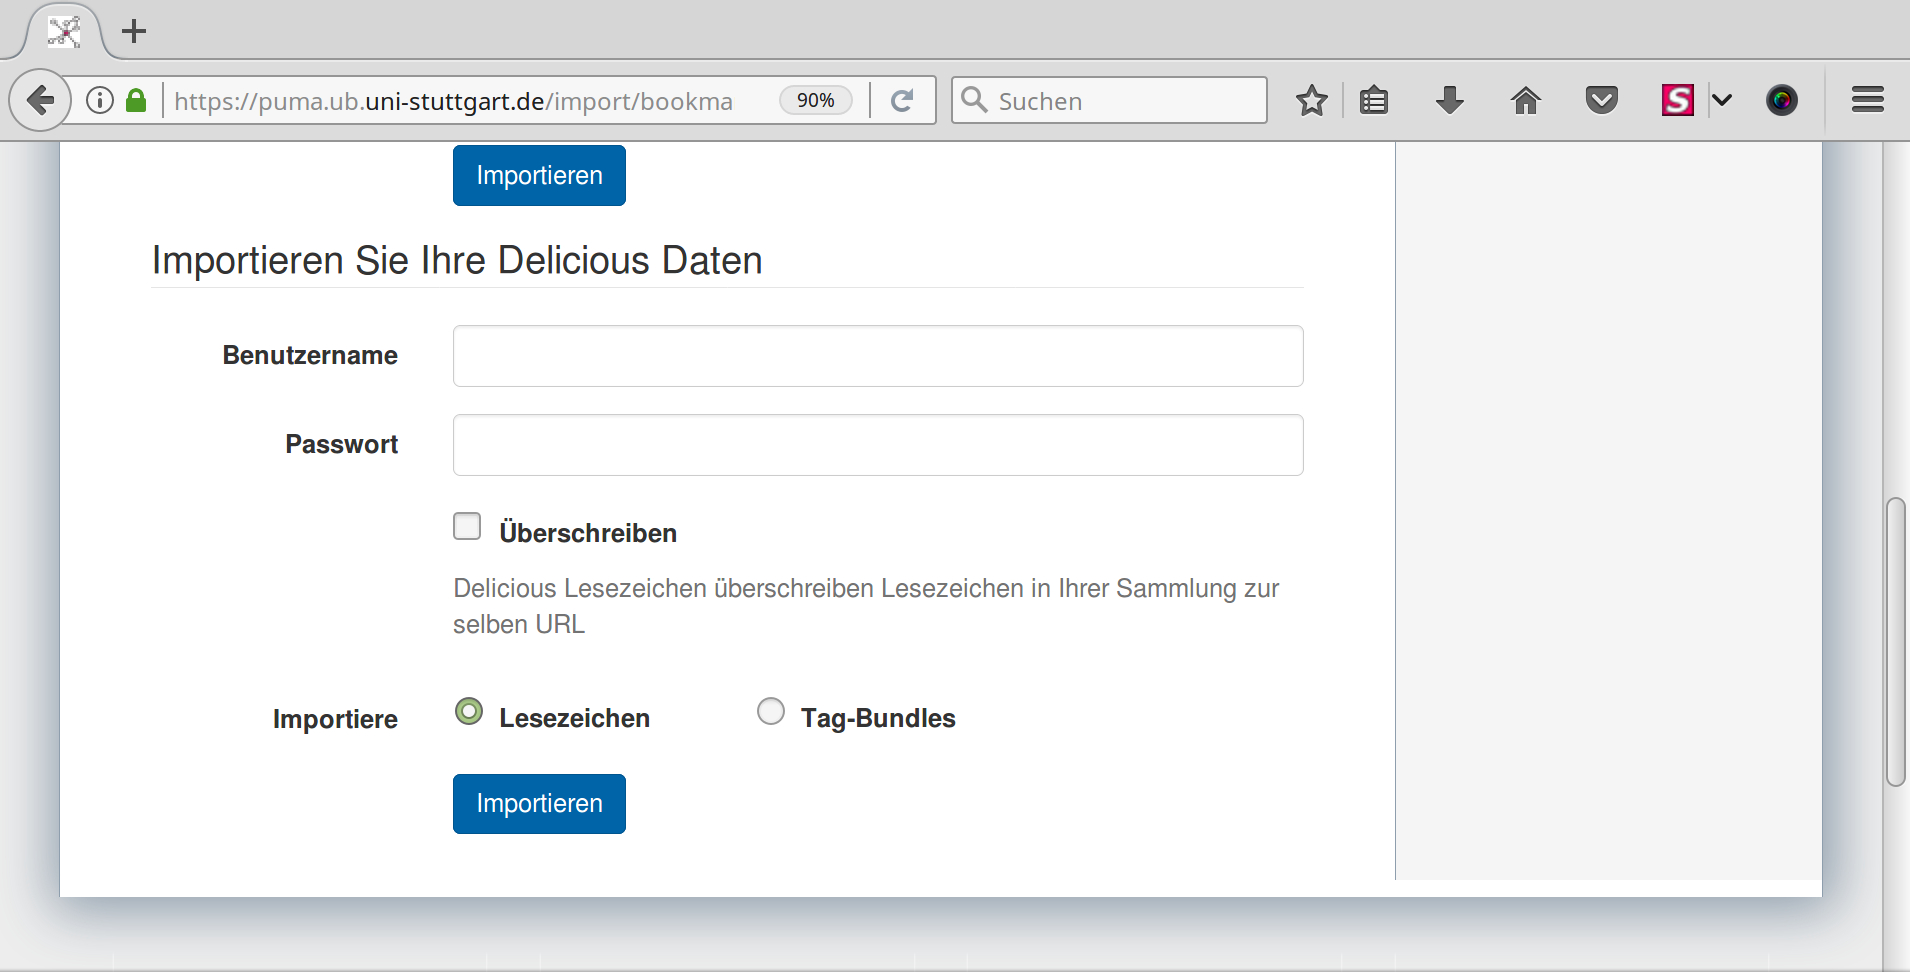
\includegraphics[width=11cm]{Bilder/Kapitel5/Delicious_Daten}}
 \caption{Delicious Daten}
 \label{fig:deliciousDaten}
\end{figure} 
\section{Publikationen importieren}
\label{sec:publikationenImportieren}
PUMA ermöglicht Ihnen bereits bestehende BibTeX- oder EndNote-Datei hochladen. Vergewissern Sie sich hierbei, dass Sie die korrekte Kodierung gewählt haben. Falls die Datei nur wenige Einträge enthält, können Sie diese auf der folgenden Seite bearbeiten. 
\begin{enumerate}
	\item Klicken Sie auf das Feld \enquote{Durchsuchen} und laden die entsprechende Datei hoch. 
	\item Wählen Sie die Sichtbarkeit aus.
	\item In den \enquote{Erweiterte Einstellungen} können Sie anschließend noch die Datei vor dem Import bearbeiten und festlegen, ob ein älterer Eintrag überschrieben werden soll, wenn der importierte Eintrag die gleiche Publikation referenziert wie ein bereits existierender Eintrag.
	\item Klicken Sie anschließend auf \enquote{Weiter}, um den Eintrag zu vervollständigen und zu speichern.
\end{enumerate}
\begin{figure}[h!]
 \centering
 \fbox{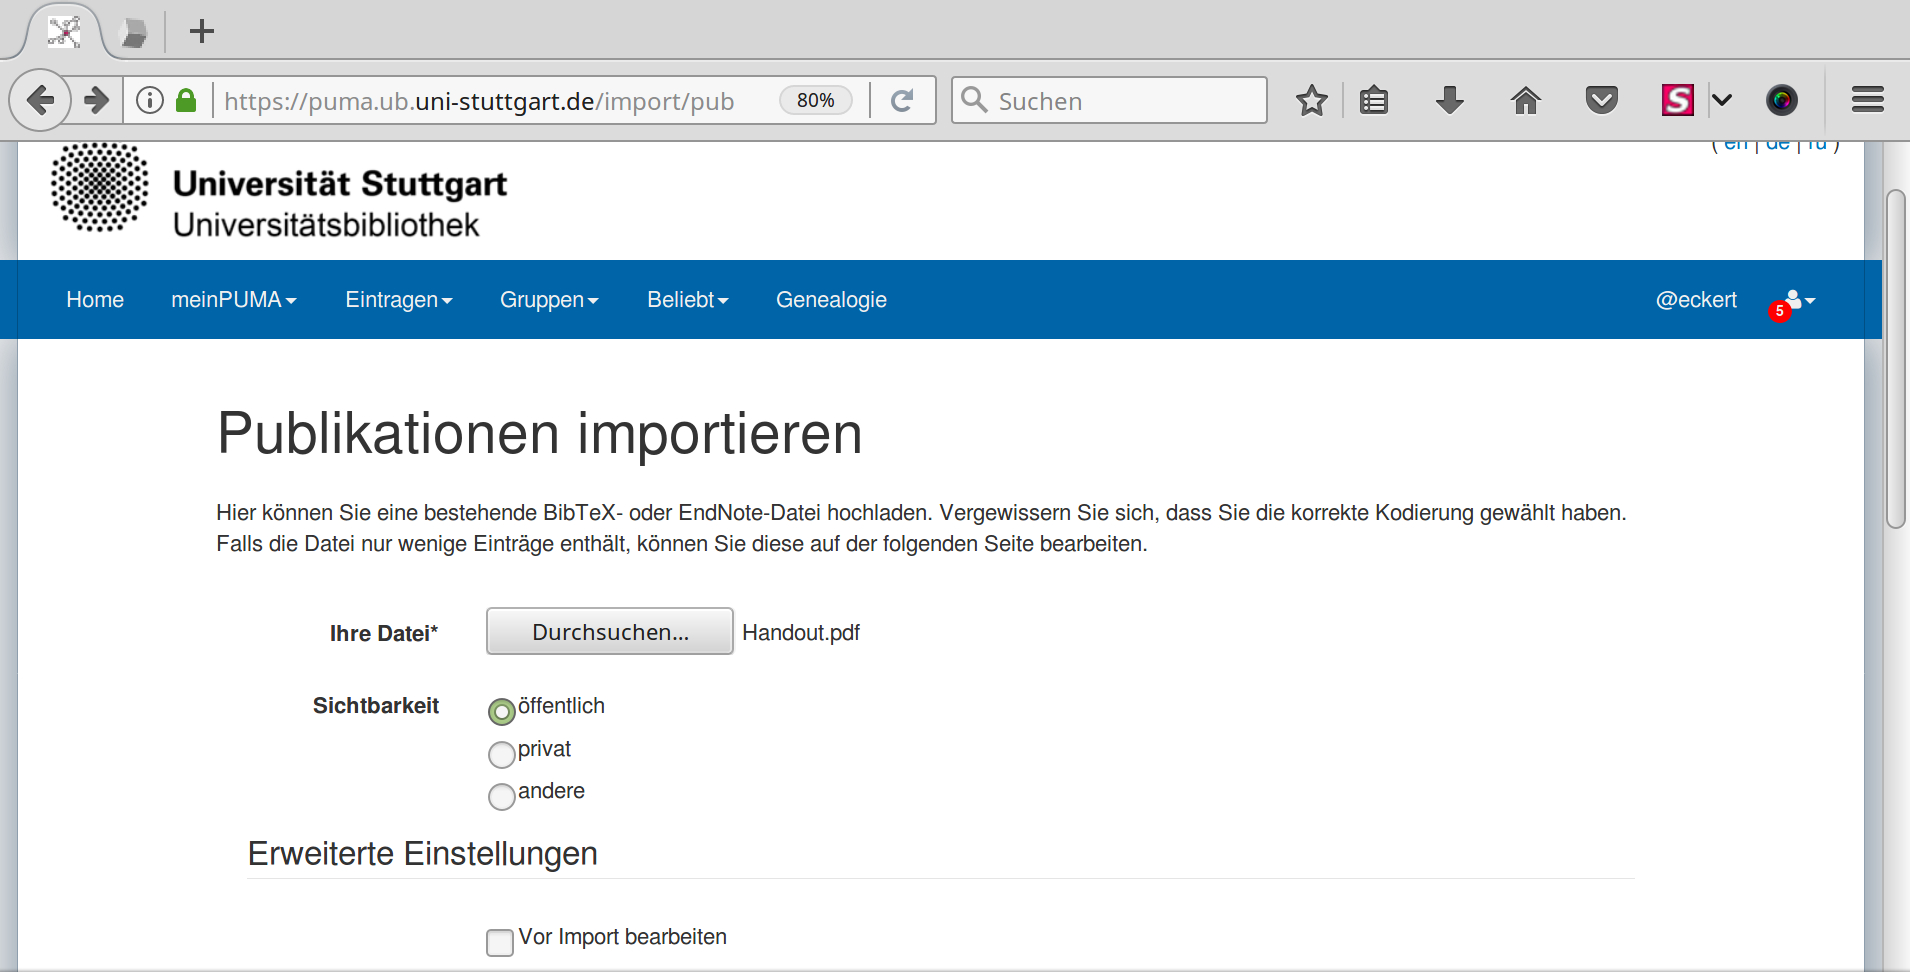
\includegraphics[width=11cm]{Bilder/Kapitel5/Publikationen_importieren}}
 \caption{Publikationen importieren}
 \label{fig:publikationenImportieren}
\end{figure}  



  
\section{Bookmarklet-Buttons für Ihre Lesezeichen-Leiste}\label{sec:button}
Die Bookmarklet-Buttons\index{Bookmarklet-Buttons} ermöglichen Ihnen ein schnelles Arbeiten mit PUMA, während Sie im Internet unterwegs sind. Sie vereinfachen Ihnen das Eintragen von Publikationen und Lesezeichen und gelangen mit dem PUMA-Home Bookmarklet-Button direkt zu PUMA. Ziehen Sie die Buttons\footnote{\url{https://puma.ub.uni-stuttgart.de/buttons}} einfach in Ihre Lesezeichen-Leiste und schon können Sie loslegen.
\begin{figure}[h!]
 \centering
 \fbox{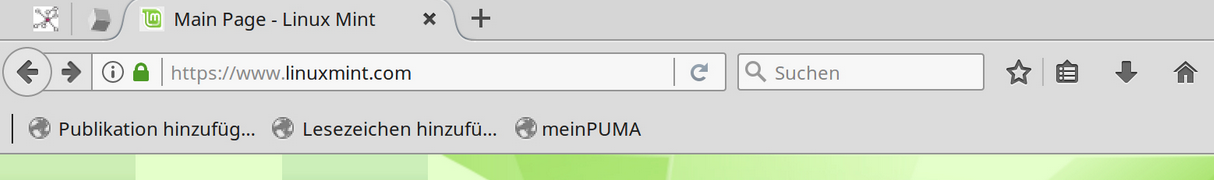
\includegraphics[width=11cm]{Bilder/Kapitel5/Bookmarklet-Buttons}}
 \caption{Bookmarklet-Buttons}
 \label{fig:bookmarkletButtons}
\end{figure} 
\section{PUMA-Browser-Add-ons\index{Add-ons}}\label{sec:addon}
Erweitern Sie Ihren Browser mit diesem Add-on um drei nützliche PUMA-Schaltflächen: Mit einem Klick zu PUMA, eine Publikation oder ein Lesezeichen speichern.\newline
\begin{enumerate}
\item Klicken Sie rechts oben im Firefox-Browser auf das Menü.
\begin{figure}[h!]
 \centering
 \fbox{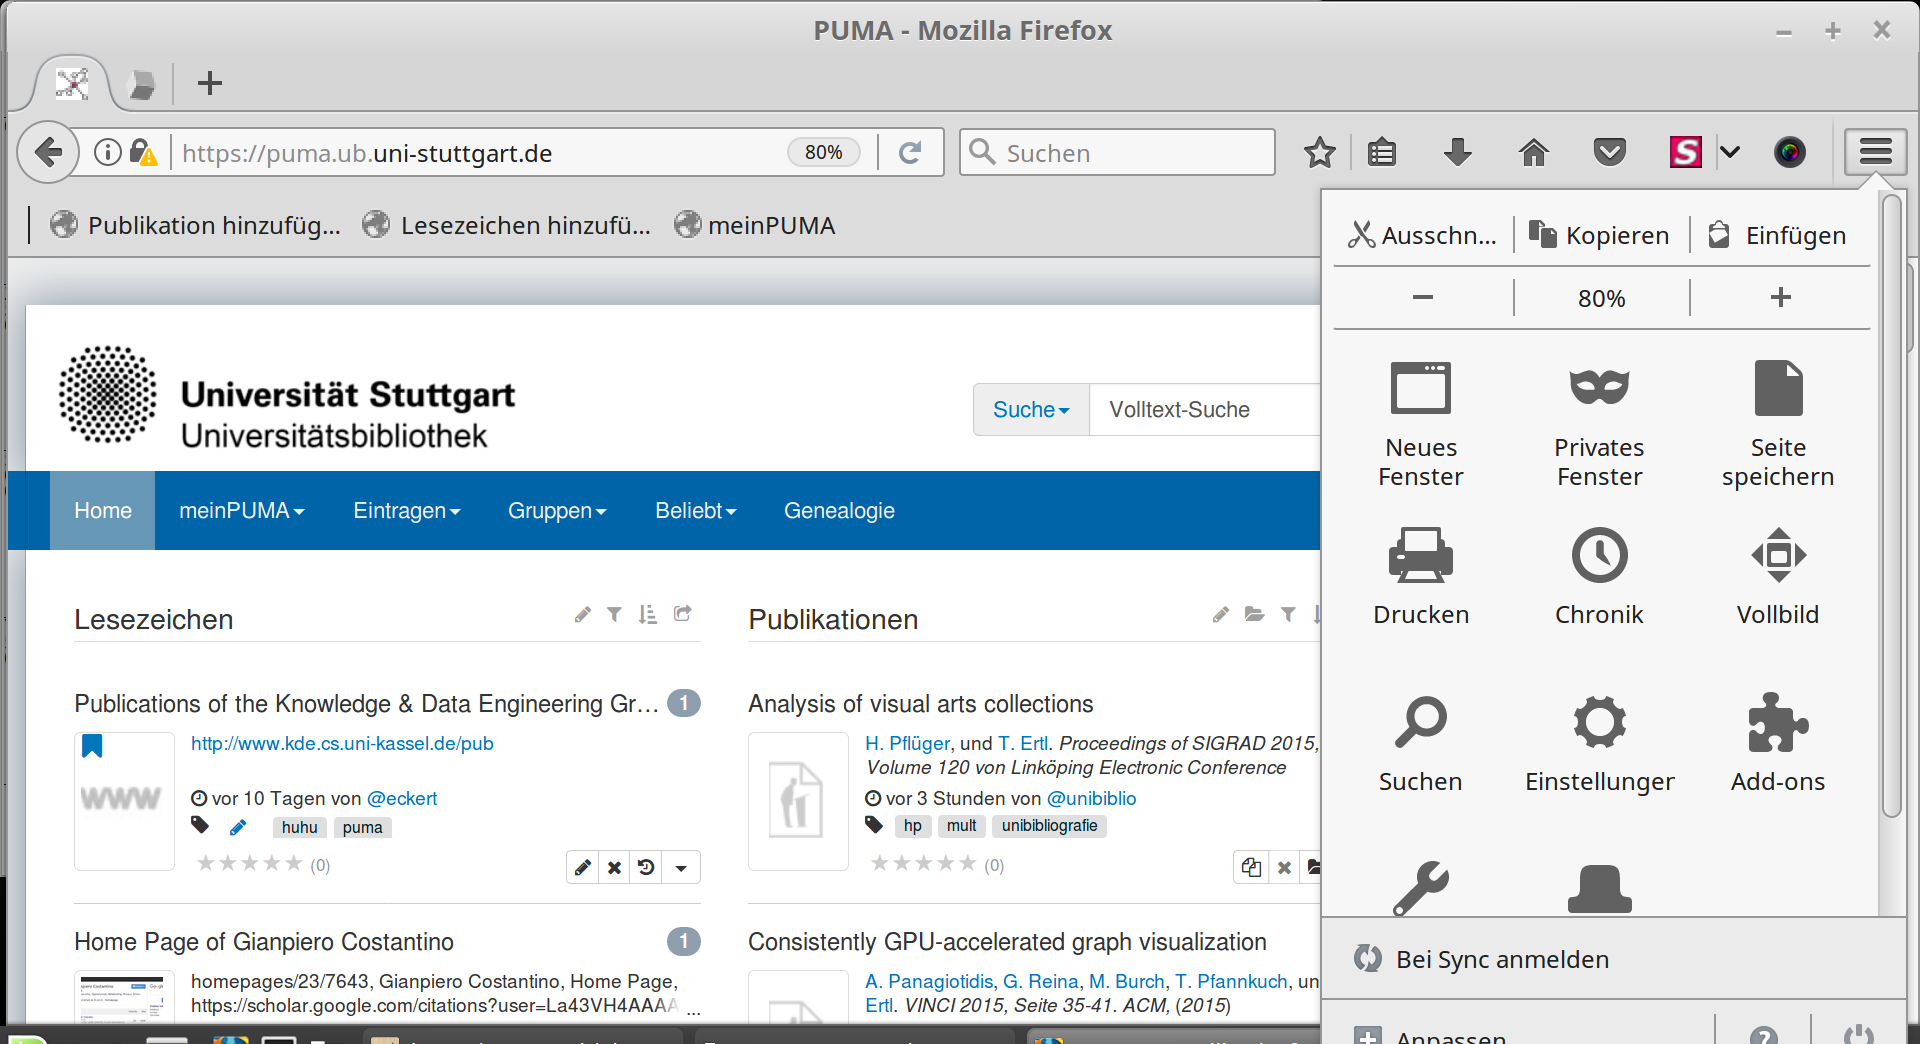
\includegraphics[width=11cm]{Bilder/Kapitel5/Menue_Firefox}}
 \caption{Firefox-Browser}
 \label{fig:firefoxBrowser}
\end{figure} 
\item Es öffnet sich das Menü, wählen Sie den Reiter \enquote{Add-ons} aus. 
\item Geben Sie in die Suchleiste oben rechts \enquote{puma} ein.
\item Es erscheint das Add-on \enquote{PUMA Buttons}. Installieren Sie die Buttons (Version 1.6.2).
\begin{figure}[h!]
 \centering
 \fbox{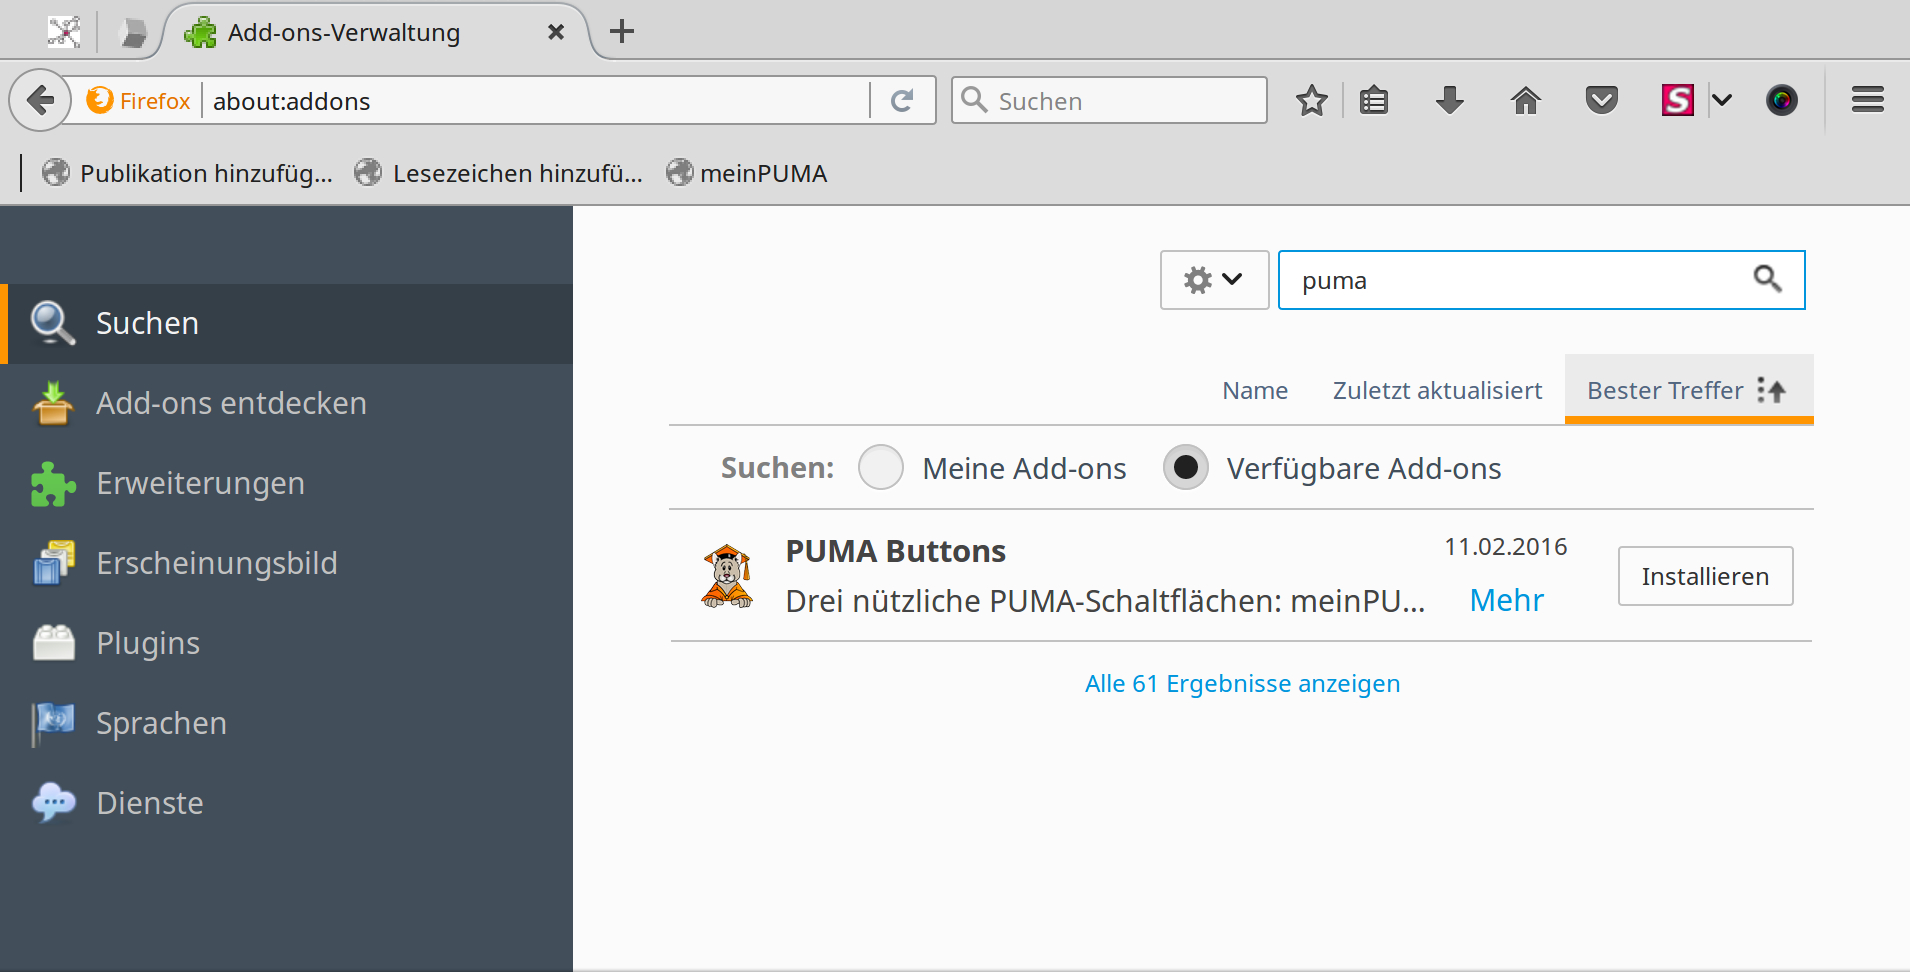
\includegraphics[width=11cm]{Bilder/Kapitel5/PUMA_Buttons}}
 \caption{Puma Buttons}
 \label{fig:pumaButtons}
\end{figure} 
\item Klicken Sie anschließend auf \enquote{mehr} und scrollen auf der Seite runter bis zum Abschnitt \enquote{Instanz wechseln}. 
\item Durch das Klicken auf \enquote{Instanz wechseln} öffnet sich eine Übersicht über alle verfügbaren PUMAs. Wählen Sie  \enquote{UB Stuttgart} aus und speichern Ihre Wahl.
\item Falls die Buttons nicht sofort in der Taskleiste neben dem Menüsymbol  erscheinen, schließen Sie Firefox. Beim erneuten Öffnen des Firefox-Browsers wurden die Buttons eingerichtet.
\end{enumerate}
\section{Ablage}
\label{sec:ablage}
Die Ablage\index{Ablage} ermöglicht es Ihnen eigene und fremde Publikationen vorzumerken. Sie können so in der Ablage aktuelle Literaturlisten zusammenstellen.
\newline
Publikationen in Ablage aufnehmen: %Screenshot
\begin{enumerate}
    \item Klicken Sie auf das Symbol \enquote{Diese Publikation zur Ablage hinzufügen}.
    \item Die Publikationen gelangen direkt in die Ablage. Zur Ablage gelangen Sie über das Personensymbol.
\end{enumerate}
\begin{figure}[h!]
 \centering
 \fbox{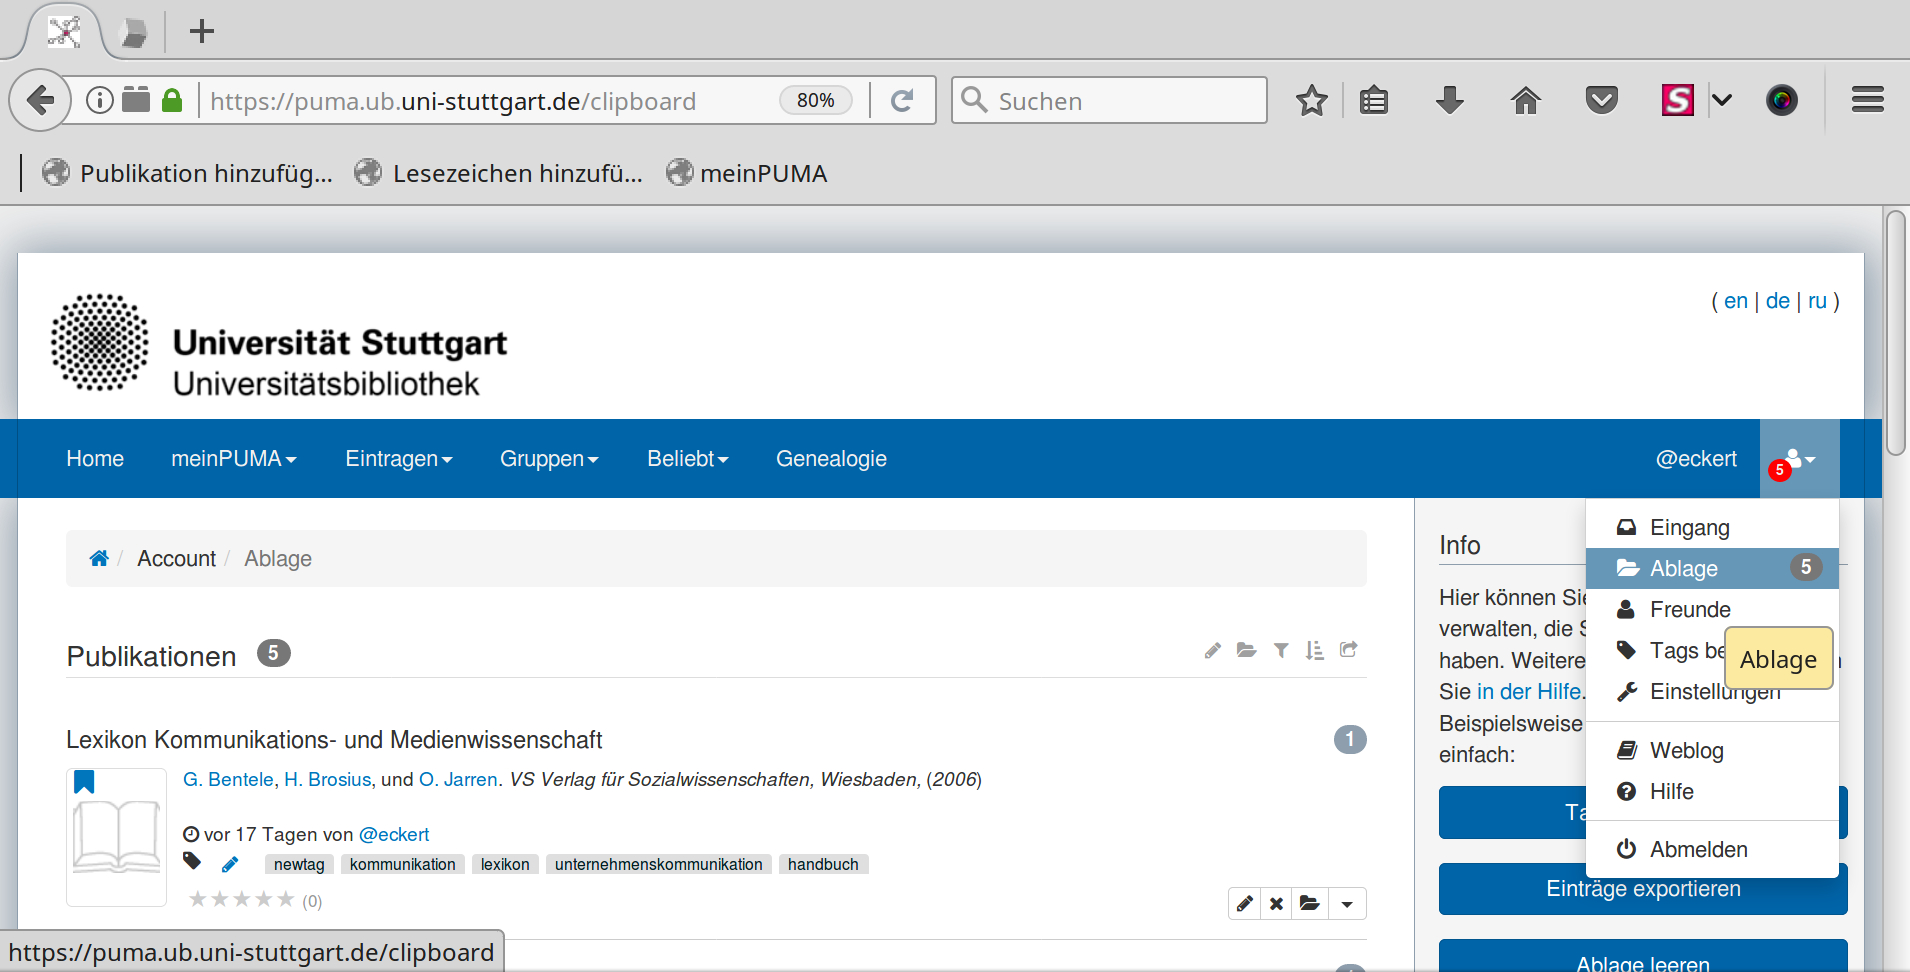
\includegraphics[width=11cm]{Bilder/Kapitel5/Ablage}}
 \caption{Die Ablage}
 \label{fig:ablage}
\end{figure} 
Falls Sie die vorgemerkten Publikationen nicht mehr in der Ablage haben möchten können Sie diese löschen, indem Sie auf das schwarze \enquote{X} (diese Publikation aus Ihrer Sammlung löschen) klicken.\newline
%\begin{wrapfigure}{l}{5cm}
\begin{tip}Wenn Sie die Publikation in der Ablage löschen ist diese gleichzeitig auch in Ihrer Sammlung gelöscht und kann nicht wiederhergestellt werden.
\end{tip}
%\end{wrapfigure}

Eine andere Möglichkeit ist das Leeren der Ablage. Dies erreichen Sie, indem Sie auf der rechten Seite auf das blaue Feld \enquote{Ablage leeren} klicken. In diesem Fall werden die Publikationen aus der Ablage entfernt, sind aber in Ihrer Sammlung noch vorhanden.
\section{Freischalten erweiterter Funktionen}
\label{sec:freischaltenErweiterterFunktionen}
Bei PUMA gibt es die Unterscheidung zwischen einfachen\index{Funktionen!Einfache} und erweiterten Funktionen\index{Funktionen!Erweiterte}. In den Grundeinstellungen stehen jedem Nutzer, bei dessen Anmeldung bei PUMA, die einfachen Funktionen zur Verfügung. Durch das Freischalten der erweiterten Funktionen kommen weitere Funktionen hinzu, sodass Sie mehr Möglichkeiten haben, PUMA zu nutzen.  Wenn Sie die erweiterten Funktionen freischalten möchten, gehen Sie wie folgt vor:
\begin{enumerate}
    \item Klicken Sie auf das Personensymbol. Ein Dropdown-Menü öffnet sich, klicken Sie auf \enquote{Einstellungen}.
    \item Es öffnet sich die Einstellungs-Seite. Klicken Sie oben auf den Reiter \enquote{Einstellungen}.
    \item Unter dem Bereich \enquote{Layouts Ihrer Tagbox und Ihrer Eintragslisten} befindet sich das Feld \enquote{Erscheinungsbild}. Sie können nun zwischen den Standardeinstellungen \textit{Erweitert} (Alle Optionen werden stets angezeigt) oder \textit{Einfach} (Einige \enquote{Experten}-Optionen werden standardmäßig nicht angezeigt) wählen.
    \begin{figure}[h!]
 \centering
 \fbox{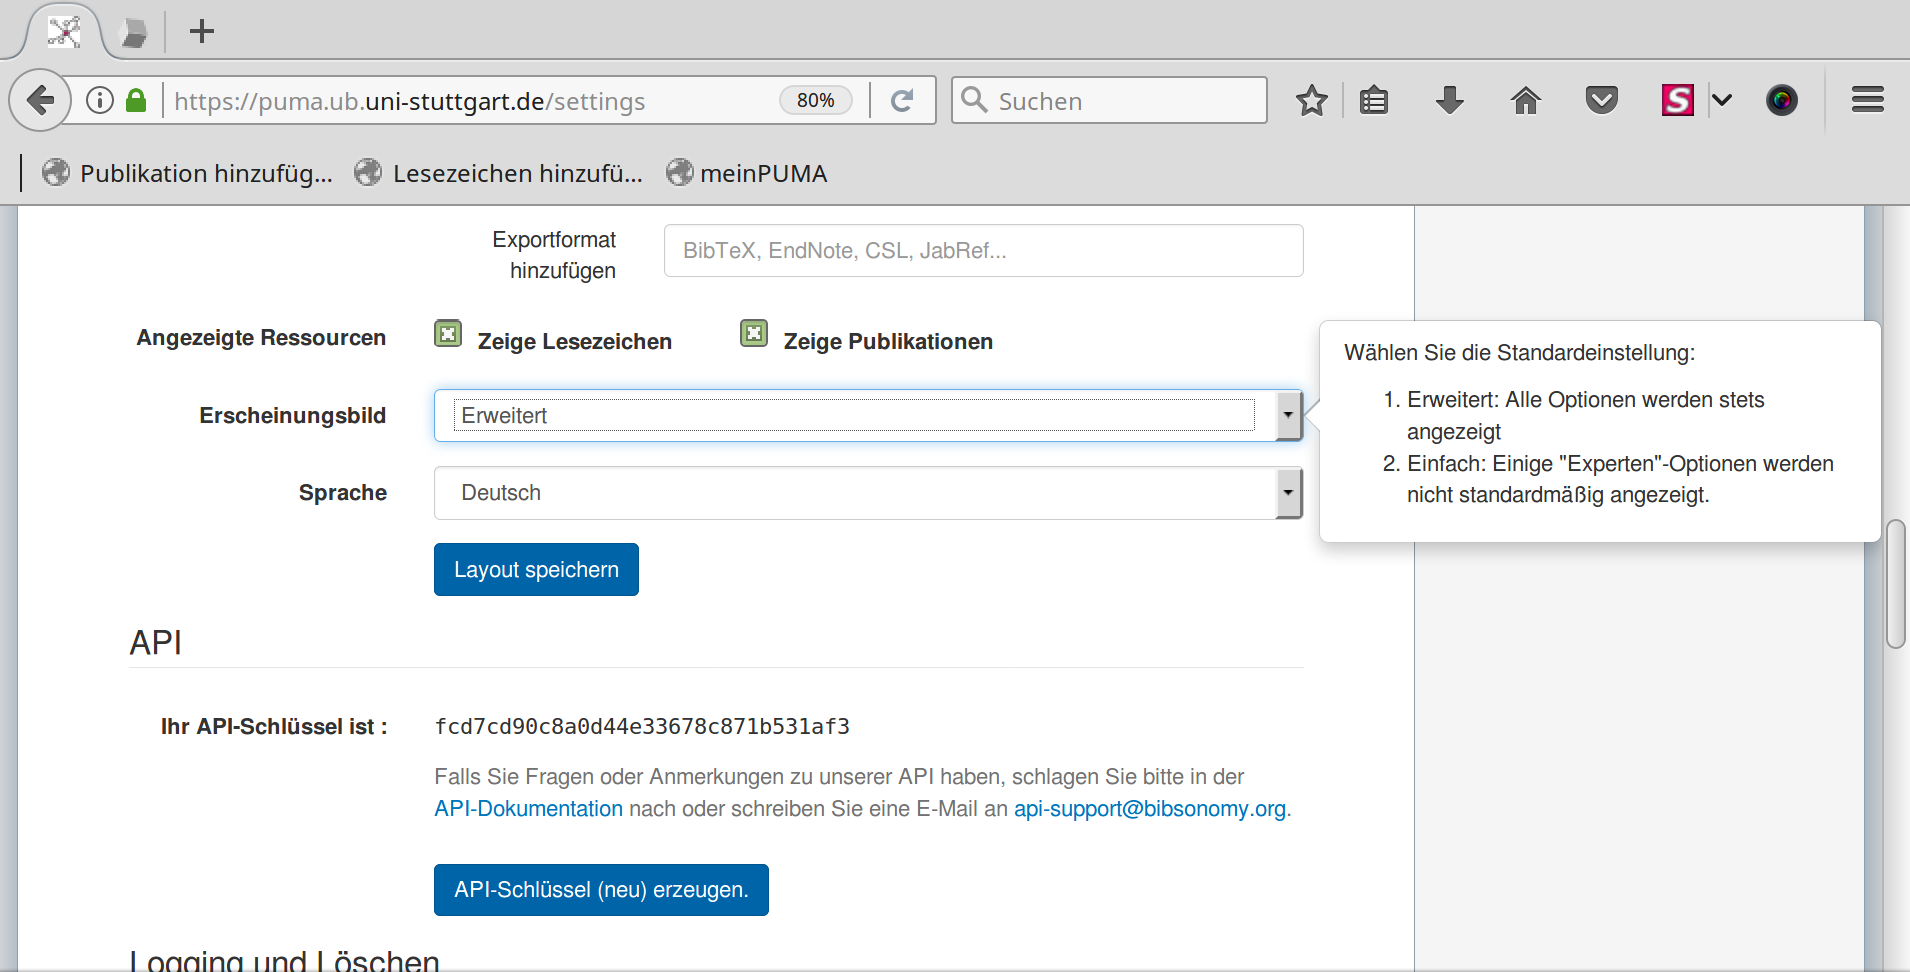
\includegraphics[width=11cm]{Bilder/Kapitel5/Erweiterte_Funktionen}}
 \caption{Erweiterte Funktionen}
 \label{fig:erweiterteFunktionen}
\end{figure} 
    \item Klicken Sie anschließend auf \enquote{Layout speichern}, um Ihre Änderung zu sichern.
\end{enumerate}
\section{Konto auflösen}
\label{sec:kontoAufloesen} 
\subsection{Konto löschen}\index{Konto!löschen} \label{subsec:kontoAufloesen}
\subsection{Ausscheiden aus der Uni}\index{Konto!auflösen} \label{subsec:kontoLoeschen}
